% ******************************* PhD Thesis Template **************************
% Please have a look at the README.md file for info on how to use the template

\documentclass[a4paper,12pt,times,numbered,print,index]{PhDThesisPSnPDF}
\RequirePackage{listings}

% ******************************************************************************
% ******************************* Class Options ********************************
% *********************** See README for more details **************************
% ******************************************************************************

% `a4paper'(The University of Cambridge PhD thesis guidelines recommends a page
% size a4 - default option) or `a5paper': A5 Paper size is also allowed as per
% the Cambridge University Engineering Deparment guidelines for PhD thesis
%
% `11pt' or `12pt'(default): Font Size 10pt is NOT recommended by the University
% guidelines
%
% `oneside' or `twoside'(default): Printing double side (twoside) or single
% side.
%
% `print': Use `print' for print version with appropriate margins and page
% layout. Leaving the options field blank will activate Online version.
%
% `index': For index at the end of the thesis
%
% `draftclassic': For draft mode without loading any images (same as draft in book)
%
% `draft': Special draft mode with line numbers, images, and water mark with
% timestamp and custom text. Position of the text can also be modified.
%
% `abstract': To generate only the title page and abstract page with
% dissertation title and name, to submit to the Student Registry
%
% `chapter`: This option enables only the specified chapter and it's references
%  Useful for review and corrections.
%
% ************************* Custom Page Margins ********************************
%
% `custommargin`: Use `custommargin' in options to activate custom page margins,
% which can be defined in the preamble.tex. Custom margin will override
% print/online margin setup.
%
% *********************** Choosing the Fonts in Class Options ******************
%
% `times' : Times font with math support. (The Cambridge University guidelines
% recommend using times)
%
% `fourier': Utopia Font with Fourier Math font (Font has to be installed)
%            It's a free font.
%
% `customfont': Use `customfont' option in the document class and load the
% package in the preamble.tex
%
% default or leave empty: `Latin Modern' font will be loaded.
%
% ********************** Choosing the Bibliography style ***********************
%
% `authoryear': For author-year citation eg., Krishna (2013)
%
% `numbered': (Default Option) For numbered and sorted citation e.g., [1,5,2]
%
% `custombib': Define your own bibliography style in the `preamble.tex' file.
%              `\RequirePackage[square, sort, numbers, authoryear]{natbib}'.
%              This can be also used to load biblatex instead of natbib
%              (See Preamble)
%
% **************************** Choosing the Page Style *************************
%
% `default (leave empty)': For Page Numbers in Header (Left Even, Right Odd) and
% Chapter Name in Header (Right Even) and Section Name (Left Odd). Blank Footer.
%
% `PageStyleI': Chapter Name next & Page Number on Even Side (Left Even).
% Section Name & Page Number in Header on Odd Side (Right Odd). Footer is empty.
%
% `PageStyleII': Chapter Name on Even Side (Left Even) in Header. Section Number
% and Section Name in Header on Odd Side (Right Odd). Page numbering in footer

% Uncomment to change page style
%\pagestyle{PageStyleII}

% ********************************** Preamble **********************************
% Preamble: Contains packages and user-defined commands and settings
\input{Preamble/preamble}

% ************************ Thesis Information & Meta-data **********************
% Thesis title and author information, refernce file for biblatex
% ************************ Thesis Information & Meta-data **********************
%% The title of the thesis
% \title{Writing your PhD thesis in \texorpdfstring{\\ \LaTeX2e}{LaTeX2e}}
\title{FAT-Pointer based range addresses}
%\texorpdfstring is used for PDF metadata. Usage:
%\texorpdfstring{LaTeX_Version}{PDF Version (non-latex)} eg.,
%\texorpdfstring{$sigma$}{sigma}

%% Subtitle (Optional)
% \subtitle{Using the CUED template}

%% The full name of the author
\author{Akilan Selvacoumar}

%% Department (eg. Department of Engineering, Maths, Physics)
\dept{Mathematics and Computer Sciences}

%% University and Crest
\university{Heriot Watt University}
% Crest minimum should be 30mm.
\crest{
\includegraphics[width=0.2\textwidth]{heriot-watt-university.png}}
%% Use this crest, if you are using the college crest
%% Crest long miminum should be 65mm
%\crest{\includegraphics[width=0.45\textwidth]{University_Crest_Long}}

%% College shield [optional] 
% Crest minimum should be 30mm.
%\collegeshield{\includegraphics[width=0.2\textwidth]{CollegeShields/Kings}}


%% Supervisor (optional)
%% for multiple supervisors, append each supervisor with the \newline command
%\supervisor{Prof. A.B. Supervisor\newline
%Prof. C.D. Supervisor}

%% Supervisor Role (optional) - Supervisor (default) or advisor
% \supervisorrole{\textbf{Supervisors: }}
%% if no title is desired:
% \supervisorrole{}

%% Supervisor line width: required to align supervisors
%\supervisorlinewidth{0.35\textwidth}

%% Advisor (optional)
%% for multiple advisors, append each advisor with the \newline command
%\advisor{Dr. A. Advisor\newline
%Dr. B. Advisor}
     
%% Advisor Role (optional) - Advisor (default) or leave empty
% \advisorrole{Advisors: }
%% if no title is required
% \advisorrole{}

%% Advisor line width: required to align supervisors
%\advisorlinewidth{0.25\textwidth}


%% You can redefine the submission text:
% Default as per the University guidelines:
% ``This dissertation is submitted for the degree of''
\renewcommand{\submissiontext}{Year 2 progression report of:}

%% Full title of the Degree
\degreetitle{Doctor of Philosophy}

%% College affiliation (optional)
% \college{King's College}

%% Submission date
% Default is set as {\monthname[\the\month]\space\the\year}
%\degreedate{September 2014} 

%% Meta information
\subject{LaTeX} \keywords{{LaTeX} {PhD Thesis} {Engineering} {Heriot Watt}}


% ***************************** Abstract Separate ******************************
% To printout only the titlepage and the abstract with the PhD title and the
% author name for submission to the Student Registry, use the `abstract' option in
% the document class.

\ifdefineAbstract
 \pagestyle{empty}
 \includeonly{Declaration/declaration, Abstract/abstract}
\fi

% ***************************** Chapter Mode ***********************************
% The chapter mode allows user to only print particular chapters with references
% Title, Contents, Frontmatter are disabled by default
% Useful option to review a particular chapter or to send it to supervisior.
% To use choose `chapter' option in the document class

\ifdefineChapter
 \includeonly{Chapter3/chapter3}
\fi

% ******************************** Front Matter ********************************
\begin{document}

\frontmatter

\maketitle

% % ******************************* Thesis Dedidcation ********************************

\begin{dedication} 

I would like to dedicate this thesis to my loving parents. \dots

\end{dedication}


% \include{Declaration/declaration}
% \include{Acknowledgement/acknowledgement}
% ************************** Thesis Abstract *****************************
% Use `abstract' as an option in the document class to print only the titlepage and the abstract.
\begin{abstract}
There has been a lot work done in the areas of slim down kernels, OS paradigms which treat a multi-core machine as network of independent cores 
and specialized hardware which could provide certain security features. While they have been heavily independently worked on. The major aims for 
the following research would be to combine all 3 of them to together and address the potential benefits from such an approach. The year 1 report 
does a survey of implementations done in the areas Uni-kernels, Multi-kernels and TAG based architectures. Based on these surveys, comes up
with the research aims for the following PhD. A timeline is provided with the detailed plan for the following research.
\end{abstract}


% *********************** Adding TOC and List of Figures ***********************

\tableofcontents

% \listoffigures

% \listoftables

% \printnomenclature[space] space can be set as 2em between symbol and description
%\printnomenclature[3em]

%\printnomenclature

% ******************************** Main Matter *********************************
\mainmatter

\chapter{Introduction}
In the dynamic landscape of computing, the pursuit of optimal performance is a constant endeavor, 
especially as applications evolve to handle increasingly complex workloads. 
One critical aspect influencing performance is memory management, where efficient 
utilization of resources is paramount. Translation Lookaside Buffers (TLBs) play a 
pivotal role in this regard, expediting memory access by storing recently accessed memory translations.
However, as applications grow in size and complexity, the capacity of TLBs often struggles to 
keep pace, leading to performance bottlenecks. To address this challenge, researchers have 
turned to innovative solutions, one of which involves harnessing the benefits of huge pages.
Huge pages, also known as large pages, allow for the allocation of memory in significantly 
larger chunks compared to traditional small pages. By reducing the number of TLB entries 
needed to access a given amount of memory, huge pages offer a potential avenue for optimizing 
TLB utilization and thereby enhancing overall system performance.

Simultaneously, advancements in hardware-level security, such as the Capability Hardware 
Enhanced RISC Instructions (CHERI) architecture, present additional opportunities for 
performance enhancement. CHERI's capability-based addressing approach not only strengthens 
system security by tightly controlling memory access but also provides avenues for 
accelerating memory management operations.

In this context, the integration of huge pages into memory management 
strategies alongside capability-based addressing in architectures like 
CHERI offers a compelling synergy. By optimizing TLB utilization through the 
utilization of huge pages and leveraging the security features of capability-based addressing, 
significant performance improvements can be realized. This approach not only enhances 
system security but also accelerates memory access.

% TODO: 
% - Add references for FlexPointer, Range Memory Mapping (RMM), Direct Segment and Huge Pages
\subsection{TLB based approaches}
Efficient memory management, particularly in the context of 
Translation Lookaside Buffer (TLB) optimization, has been a focal point of 
research and development within computer architecture. Various techniques have been 
proposed to mitigate TLB-related bottlenecks and improve overall system performance.

\subsubsection{Huge Pages:}
This is used to map a very large region of memory to a 
single entry. This small/large region of memory is physically
contiguous. Most implementations of huge pages \cite{panwar_hawkeye_2019} are size
aligned, For example for the x86 architecture the huge pages 
size are 4KB, 2MB and 1GB pages. 
% \subsection{Tailored page sizes}
% TODO later
% \subsection{TLB coalescing}
% This leverages the default OS allocator behavior to pack
% multiple PTEs into a single TLB entry.

\subsubsection{Segment:}
A segment\cite{basu_efficient_nodate} can be viewed as mapping between contiguous virtual
memory and contiguous physical memory. The property of a 
segment allows it to be larger than a page. Direct Segment allows the user to set a single segment
for an application. Two registers are added to mark the start
and end of the segment. Any virtual address within this region
can be translated by adding the fixed offset between the virtual
and physical address.

\subsubsection{Range Memory Mapping (RMM):}
RMM\cite{karakostas_redundant_2015} introduces the concept of adding an additional range table.
For large allocations RMM eagerly allocates contiguous physical pages.
The following allocations creates large memory ranges that are
both virtually and physically contiguous. RMM builds on the concept
of Direct segment by adding offset to translate a virtual address 
to physical address. RMM compares address with range boundaries 
to decide which range it belongs to. RMM queries the range table 
ofter an L1 TLB miss.

\subsubsection{FlexPointer:}
FlexPointer\cite{chen_flexpointer_2023} is based on the RMM\cite{karakostas_redundant_2015} paper. FlexPointer
does eagerly allocate pages which are physically contiguous and stores the ID to translate a virtual address 
to physical address on the remaining unused bits on the 64 bit virtual address. 
The paper contribution mentions shifting the TLB lookup to an earlier stage to improve
latency of accessing the TLB entries. FlexPointer immediate queries the 
range TLB for translations rather than the RMM paper which waits for the L1 TLB miss.

\subsection{CHERI}
A capability functions as a token that provides the holder with the authority to 
execute specific actions. By carefully managing who possesses these capabilities, 
it is possible to enforce security measures, such as ensuring that a particular
section of software can only read from a designated range of memory addresses.

The concept of cap  abilities has a rich history in computer science, tracing 
back to early systems designed to enhance security and manage resources effectively.
For instance, foundational work discussed in sources like \cite{noauthor_capability-based_nodate} offers a comprehensive 
narrative on the evolution of capability architectures. This historical perspective 
can be further enriched by incorporating insights from more recent studies, 
such as those found in \cite{miller_towards_nodate}.

CHERI (Capability Hardware Enhanced RISC Instructions)\cite{woodruff_cheri_2019} represents a modern embodiment of this 
long-standing idea. It introduces more granular control over permissions, allowing for finer 
distinctions in what actions can be performed and by whom. Moreover, CHERI is designed to integrate 
seamlessly with contemporary processor instruction sets, ensuring that these advanced security 
features can be implemented on modern hardware platforms. This adaptation not only revitalizes 
the capability concept but also significantly enhances its applicability and effectiveness 
in current computing environments.
\chapter{Fat Pointer Based Range Addresses}

\ifpdf
    \graphicspath{{Fat-Pointer-Based-Range-Address/Figs/Raster/}{Fat-Pointer-Based-Range-Address/Figs/PDF/}{Fat-Pointer-Based-Range-Address/Figs/}}
\else
    \graphicspath{{Fat-Pointer-Based-Range-Address/Figs/Vector/}{Fat-Pointer-Based-Range-Address/Figs/}}
\fi


FAT-Pointers based range addresses, combined with the capabilities of the CHERI (Capability Hardware Enhanced RISC Instructions) 
architecture, introduce robust memory safety and security features by incorporating additional metadata 
with memory pointers. This enhanced architecture utilizes concepts such as FlexPointer, 
Range Memory Mapping (RMM) to manage memory effectively.

Range addresses play a pivotal role within this framework, defining memory 
regions bounded by a starting address (Upper) and an ending address (Lower). 
These range addresses are encoded within FAT-pointers, allowing for precise 
control over memory regions.

The functionality of ranges encompasses several key aspects:
\begin{itemize}
\item \textbf{Creation of Physically Contiguous Memory Ranges}:
By defining memory regions that are physically contiguous, systems can 
achieve optimal memory access patterns, enhancing performance and efficiency.
\item \textbf{Encoding Ranges as Bounds to the Pointer}:
Integrating range bounds directly into FAT-pointers enables the architecture 
to enforce memory access restrictions at the pointer level thus allowing 
tracking of memory ranges on a pointer level.
\item \textbf{Instrumenting Block-Based Allocators with Physically Contiguous Memory}:
The integration of range-based memory concepts into memory allocation systems, such as block-based 
allocators, facilitates the efficient management and utilization of physically contiguous memory blocks, 
mitigating issues related to memory fragmentation.
\end{itemize}

% \begin{minipage}[t]{0.4\linewidth}
\begin{figure}[h]
  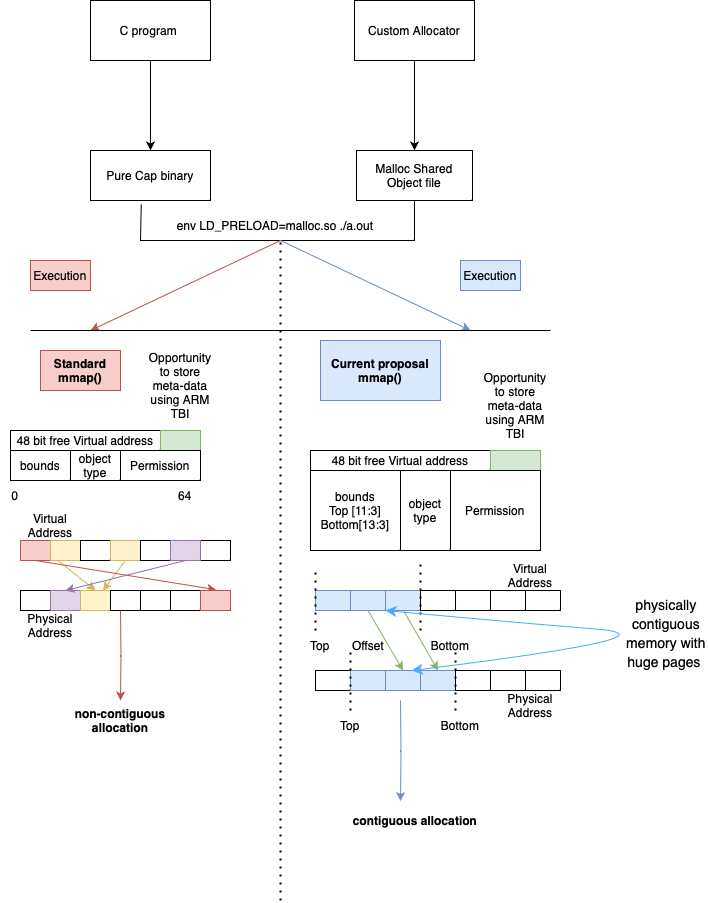
\includegraphics[width=0.6\textwidth]{diagrams/HighOverviewArchitecture24.png}
  \caption{High overview architecture}
  \label{fig:HighOverviewArchitecture}
% \end{minipage}
\end{figure}

% The figure above demonstrates the approach taken for using CHERI 
% 128bit FAT pointer scheme to allow a blocked based behavior on 
% on physically contiguous memory which is on the right against the 
% regular mmap approach which further elaborated in section (). The 
% green highlighted refers to the excess space available between 
% the 48th and 64th bit which can be used to store more meta-data which 
% is elaborated in the future work section().


Figure \ref{fig:HighOverviewArchitecture} illustrates the methodology employed to leverage the CHERI 
128-bit FAT-pointer scheme for facilitating block-based memory management
 on physically contiguous memory, which is depicted on the right side of the figure. 
 This technique contrasts with the conventional mmap approach.

In figure \ref{fig:HighOverviewArchitecture}, the green-highlighted section marks the unused space between the 48th and 64th bits
within the FAT-pointer. This area of unused bits presents an opportunity to store additional metadata,
potentially enhancing the capabilities of the memory management system. 
Here we explore how this additional metadata storage could be used to further optimize memory allocation.

% By employing the CHERI 128-bit FAT-pointer scheme, the approach depicted aims to streamline the management of memory blocks, ensuring they are physically contiguous. This is in contrast to the traditional mmap approach, which typically does not guarantee physical contiguity of allocated memory regions.


\subsection{Range creation and huge pages}
% \begin{minipage}[t]{0.4\linewidth}
\begin{figure}[h]
  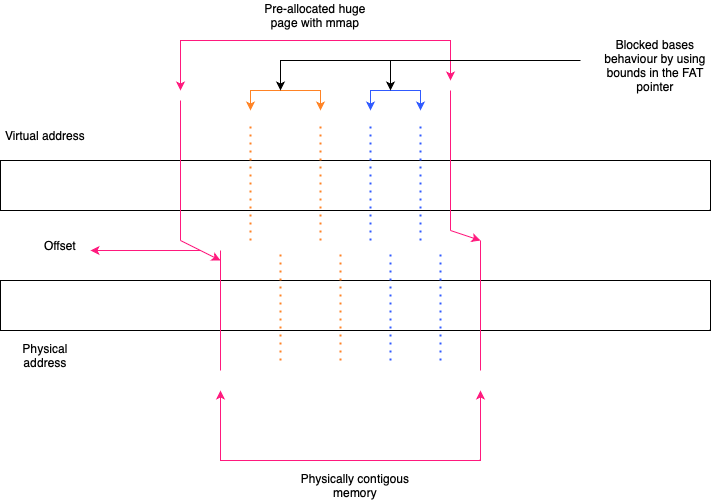
\includegraphics[width=0.8\textwidth]{diagrams/AllocationOverview24.png}
  \caption{Range of memory}
  \label{fig:RangeOfMemory}
\end{figure}
% \end{minipage}

% Ranges of memory are created based on bounds encoded to the FAT-Pointer based on the CHERI 128 bit 
% bounds compressed scheme. The Chuck between the specified upper and lower bounds are always physically
% contiguous. In the following implementation an arbitrary size huge page is initially allocated and within 
% this huge page custom size memory is allocated using a custom written mmap function which overwrites the existing block 
% based mmap function. Once memory is physically allocated using the custom mmap function call then bounds are set to it for tracking 
% the block of memory instead of using the TLB. 

In this implementation, memory ranges are established using bounds encoded within the FAT-pointer, adhering 
to the CHERI 128-bit bounds compression scheme\cite{woodruff_cheri_2019}. The memory chunk defined by the upper and lower bounds is 
always physically contiguous. Initially, a huge page of arbitrary size is allocated. Within this huge page, 
custom-sized memory segments are allocated using a custom-designed mmap function, which overrides the existing 
block-based mmap function. Once the memory is physically allocated through this custom mmap function, bounds 
are set to track the memory block, eliminating the need for traditional TLB usage for this purpose. Traditional TLB usage 
involves maintaining numerous TLB entries, often supplemented by an L2 TLB and other hierarchical structures, 
to translate virtual addresses to physical addresses. This approach requires multiple entries to handle various 
memory segments, leading to increased overhead and complexity in address translation. Conversely, 
the current approach streamlines this process by using a single TLB entry to translate multiple
 addresses within a contiguous memory range. This reduces the number of required TLB entries, 
 simplifying the translation process and improving efficiency. By consolidating address translations 
 into a single TLB entry, this method minimizes the overhead associated with managing numerous TLB entries 
 and leverages the bounds encoded within the FAT-pointer for efficient memory tracking and access. 
 This approach allows for precise and efficient memory management within the allocated huge page. 


%  The figure mentioned above demonstrates a simple use-case were the dark pink line refers to a huge page and 
%  the orange and blue lines are 2 equivalent to 2 Malloc calls allocating memory in different regions which in turn
%  emulates a block based memory allocator within a huge page using the bounds encoded in the FAT-Pointer.
\smallskip\noindent
Figure \ref{fig:RangeOfMemory} illustrates a straightforward use-case in which the dark pink line represents a single, 
large contiguous memory area, or huge page. Within this huge page, the orange and blue lines indicate 
two separate memory allocations equivalent to invoking malloc twice to allocate memory in distinct regions. 
This scenario simulates a block-based memory allocator operating within the confines of the huge page. 
The allocations leverage the bounds encoded in the FAT-pointer, ensuring tracking and efficient 
management of the allocated memory regions. By using the FAT-pointer bounds, this method maintains the 
integrity and contiguity of the allocated blocks within the huge page.

% This is done via the FreeBSD kernel Contiguous memory allocator. 

% \subsection{Fragmentation}
% The problem with standard allocators which are physically contiguous
% is that fragmentation is eminent since 
% Fragmentation is handled by using bounds as a mechanism to allocate in a block-based manner.
% Bounds are used to seek through Physically contigous 
% \subsection{Allocation with huge pages}

\subsection{Software Stack}
\begin{figure}[h]
% \begin{minipage}[t]{0.4\linewidth}
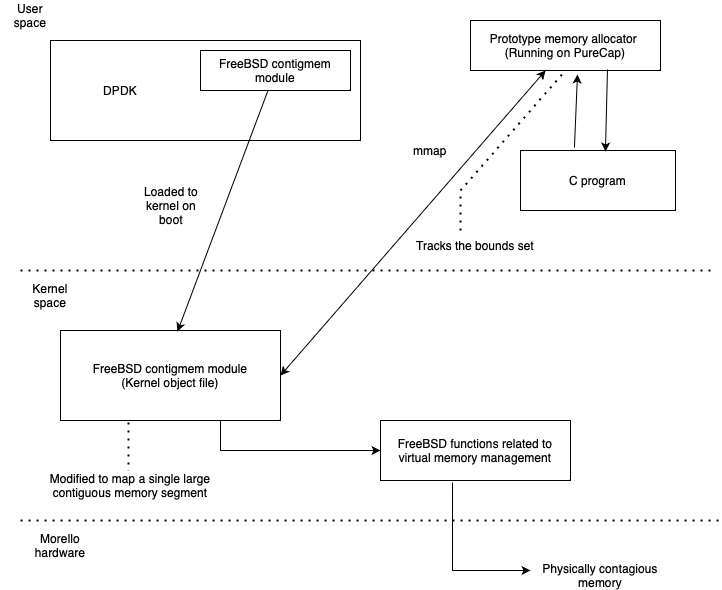
\includegraphics[width=0.8\textwidth]{diagrams/SoftwareStack24.png}
\caption{Overview of the software stack}
\label{fig:SoftwareStack}
% \end{minipage}
\end{figure}

% The Software stack consists of CHERIBSD as the base operating system due to official 
% support by ARM to the Morello's performance counters. As mentioned in the figure above 
% there is a C program that is linked to the prototype memory allocator or allocators benchmarked 
% against as mentioned in section (x) as either a Shared object file at compile time or as a header 
% file for smaller memory allocators. The modified mmap function call which is designed to be physically 
% contiguous is linked to the contigmem driver which is modified from the DPDK library (reference).
% The contigmem driver is loaded on boot time and reserves arbitrary size of a huge page which is
% set based on the experiment conducted. 

The software stack is based on CHERIBSD\cite{noauthor_getting_nodate}, selected because ARM officially supports Morello's performance 
counters\cite{noauthor_arm_nodate} on this operating system. As illustrated in the figure \ref{fig:SoftwareStack}, the setup includes a C program that 
is linked to the prototype memory allocator or to various memory allocators being benchmarked, as described 
in section~\ref{chap:evaluation}(Link to evaluation section once added). This linkage can occur in two ways: either as a shared object file during compile time 
for larger allocators, or as a header file for smaller allocators, ensuring flexibility and efficiency 
in memory management.

This integration ensures that the memory allocation process is optimized for performance, leveraging the contiguity 
of memory blocks and the capabilities provided by the CHERI architecture and the Morello platform. By using the 
contigmem driver and the custom mmap function, the system achieves efficient memory allocation and tracking, 
crucial for the high-performance needs of the application.

\subsubsection{Contigmem driver from DPDK}
The custom mmap function, tailored to ensure physically contiguous memory allocation, is a key component 
of this system. This function is linked to the contigmem driver, which has been modified from the DPDK\cite{bi_dpdk-based_2016} library 
to meet the specific needs of this implementation. The contigmem driver is essential for managing large contiguous 
memory blocks and is loaded during the system boot process. It reserves a huge page of arbitrary size, with the 
size parameter set based on the requirements of the conducted experiments.

\begin{lstlisting}[language=C, caption=Contigmem driver , label=ContigInit]

MALLOC_DEFINE(M_CONTIGMEM, "contigmem", 
"contigmem(4) allocations");

static int contigmem_modevent(module_t mod, 
int type, void *arg)
{
	int error = 0;

	switch (type) {
	case MOD_LOAD:
		error = contigmem_load();
		break;
	case MOD_UNLOAD:
		error = contigmem_unload();
		break;
	default:
		break;
	}

	return error;
}

....

DECLARE_MODULE(contigmem, contigmem_mod, 
SI_SUB_DRIVERS, SI_ORDER_ANY);
MODULE_VERSION(contigmem, 1);

static struct cdevsw contigmem_ops = {
	.d_name         = "contigmem",
	.d_version      = D_VERSION,
	.d_flags        = D_TRACKCLOSE,
	.d_mmap_single  = contigmem_mmap_single,
	.d_open         = contigmem_open,
	.d_close        = contigmem_close,
};

static int
contigmem_load()
{
	....

	for (i = 0; i < contigmem_num_buffers; i++) {
		addr = contigmalloc(contigmem_buffer_size, 
           M_CONTIGMEM, M_ZERO,
		   0, BUS_SPACE_MAXADDR, 
           contigmem_buffer_size, 0);
	....
	}

    ....

error:
	for (i = 0; i < contigmem_num_buffers; i++) {
		if (contigmem_buffers[i].addr != NULL) {
			contigfree(contigmem_buffers[i].addr,
				contigmem_buffer_size, M_CONTIGMEM);
			contigmem_buffers[i].addr = NULL;
		}
		....
	}

	return error;
}

\end{lstlisting}

% The contigmem driver~\ref{ContigInit}  function is typically initialized during boot time but can be 
% loaded manually at any time using a Kernel load instruction. The cdevsw struct includes function pointers 
% that will be replaced when the driver is loaded. For example, the mmap function can be overwritten 
% when the driver is opened and used, as illustrated in the provided code snippets.

When the contigmem\_load~\ref{ContigInit} function is called, either during boot or when the Kernel module is loaded, it pre-allocates 
a segment of physically contiguous memory. This approach differs from FlexPointer\cite{chen_flexpointer_2023}, 
which allocates physically contiguous memory eagerly. The contigmem\_load function allocates memory using contigmalloc, 
which allocates physically contiguous memory initialized to zero. The cdevsw struct refers to function 
calls which would be overwritten on loading the driver. In the code snippet~\ref{ContigInit} above
the mmap function would be overwritten with contigmem\_mmap\_single if the following driver is opened and truncated
as shown in Code snippet ~\ref{MallocSample}. 

In the code snippet ~\ref{ContigMmap} the cdev\_pager\_ops refers to the operations which will be overwritten 
when called with mmap such as overwriting page faults.

% Code snippet ~\ref{ContigInit} refers to the contigmem driver function when it 
% is initially which is normally loaded during boot time but can be loaded at any 
% point of time using Kernel load instruction. The cdevsw struct refers to function 
% calls which would be overwritten on loading the driver. In the code snippet above
% the mmap function would be overwritten if the following driver is opened and truncated
% as shown in Code snippet ~\ref{MallocInit}. The contigmem\_load function is called 
% when the Kernel module is loaded and it pre-allocates a segment of physically contigous
% memory unlike FlexPointer\cite{chen_flexpointer_2023} which eagerly allocates physically
% contigous memory. The contigmalloc function call allocates physically contigous Memory
% with the value 0. 

\begin{lstlisting}[language=C, caption=Contigmem driver mmap , label=ContigMmap]

static struct cdev_pager_ops contigmem_cdev_pager_ops = {
	.cdev_pg_ctor = contigmem_cdev_pager_ctor,
	.cdev_pg_dtor = contigmem_cdev_pager_dtor,
	.cdev_pg_fault = contigmem_cdev_pager_fault,
};

static int
contigmem_mmap_single(struct cdev *cdev, vm_ooffset_t 
*offset, vm_size_t size, struct vm_object **obj, int nprot)
{
    ....
	*obj = cdev_pager_allocate(vmh, OBJT_DEVICE, 
           &contigmem_cdev_pager_ops,size, nprot, 
           *offset, curthread->td_ucred);

	return 0;
}
\end{lstlisting}



\subsubsection{Sample memory allocator design}

\begin{lstlisting}[language=C, caption=Contigmem driver mmap , label=MallocSample]
   #define FILENAME "/dev/contigmem"
   void *ptr;
   int MallocCounter;

   size_t sizeUsed;
   
   ... 

   INITAlloc(void) {

   size_t sz;
   sz = 100000000;

   int fd = open(FILENAME, O_RDWR, 0600);

    if (fd < 0) {
        perror("open");
        exit(EXIT_FAILURE);
    }

    off_t offset = 0; // offset to seek to.

    if (ftruncate(fd, sz) < 0) {
        perror("ftruncate");
        close(fd);
        exit(EXIT_FAILURE);
    }

    ptr = mmap(NULL, sz,
    PROT_READ|PROT_WRITE, MAP_SHARED,fd,0);

   // Added error handling
    if(ptr == MAP_FAILED)
    {
        perror("mmap");
        exit(EXIT_FAILURE);
    }
    MallocCounter = (int)sz;
    }

    void* malloc(size_t sz)
    {
   sz = __builtin_align_up(sz, _Alignof(max_align_t));

   // printf("%d \n", sz);
   // printf("%d Malloc counter\n", MallocCounter);

   MallocCounter -= sz;
   void *ptrLink = &ptr[MallocCounter];
   ptrLink = cheri_setbounds(ptrLink, sz);

   return ptrLink;
     
   }

   void FREECHERI(void *ptr) { 

   // get length of free from bounds
   // in the pointer
   int len = cheri_getlen(ptr);

   munmap(ptr, len);
}

\end{lstlisting}

The code snippet~\ref{MallocSample} below shows a sample memory allocator
which is a really simple implementation that initially 
in the example allocates 1GB of memory using the mmap call which calls 
the mmap function from /dev/contigmem driver. This ensures memory allocated to the physically
contiguous memory allocated in the contigmem\_load() function using the contigmem\_mmap\_single()
function call in the kernel module, uses malloc 
and free to allocate within this memory chuck. The consideration of this is to ensure that a C program needs minor changes to use the benefit
using physically contiguous memory with bounds within a segment of memory.
\chapter{Evaluation}\label{chap:evaluation}
\ifpdf
    \graphicspath{{Evaluation/Figs/Raster/}{Evaluation/Figs/PDF/}{Evaluation/Figs/}}
\else
    \graphicspath{{Evaluation/Figs/Vector/}{Evaluation/Figs/}}
\fi

To evaluate the performance of FAT-Pointer based range addresses a sample implementation we used
the morello board with CheriBSD's Benchmark ABI\cite{noauthor_benchmark_nodate} compilation mode for accurate performance recordings. 
The evaluation is to identify CheriBSD's default memory allocator SnMalloc against the prototype memory 
allocator using the contribution of this paper in terms of: 
To assess the performance of FAT-Pointer-based range addressing in the sample implementation, we utilized the 
Morello board running CheriBSD in Benchmark ABI compilation mode to ensure precise performance measurements. 
The evaluation focuses on comparing CheriBSD's default memory allocator, SnMalloc, against the prototype 
memory allocator developed in this study, with particular attention to the following aspects:

\begin{table}[!ht]
  \centering
  \begin{tabular}{|l|l|l|l|l|}
  \hline
      Metric name & type of graph & tool used & x axis & y axis \\ \hline
      DTLB L1 read & line graph & Pmcstat & Time & DTLB L1 reads (each second) \\ \hline
      DTLB L2 read & line graph & Pmcstat & Time & DTLB L2 reads (each second) \\ \hline
      DTLB walk & line graph & Pmcstat & Time & DTLB Walks (each second) \\ \hline
      L1 cache miss & line graph & Pmcstat & Time & L1 cache miss (each second) \\ \hline
      Wall clock run time & bar graph & time & Benchmarks & Time \\ \hline
  \end{tabular}
  \caption{Metrics evaluated}
\end{table}

\section{Benchmarks used}
To conduct the evaluations, we utilized the COZ\cite{curtsinger_coz_2015} benchmark suite, a well-regarded tool specifically designed 
to measure and analyze performance improvements in concurrent programs. The COZ benchmark suite provides a
robust framework for identifying bottlenecks and evaluating the performance impact of various optimization
techniques. By leveraging COZ, developers can gain precise insights into the efficiency and scalability of
their concurrent code, making it an ideal choice for rigorous performance analysis.

From the extensive set of benchmarks provided by COZ, we selected three representative C programs. 
These programs were chosen based on their relevance to common concurrent programming patterns and
their ability to effectively demonstrate the strengths and weaknesses of different optimization 
strategies. The selected programs cover a range of concurrency scenarios, ensuring a comprehensive
evaluation of performance improvements.

By implementing these modifications, we ensured that the selected C programs not only adhered to
CHERI's security model but also maintained their functional and performance characteristics. 
This allowed us to effectively use the COZ benchmark suite to analyze the performance in a CHERI-enhanced environment.

\begin{figure}[h]
  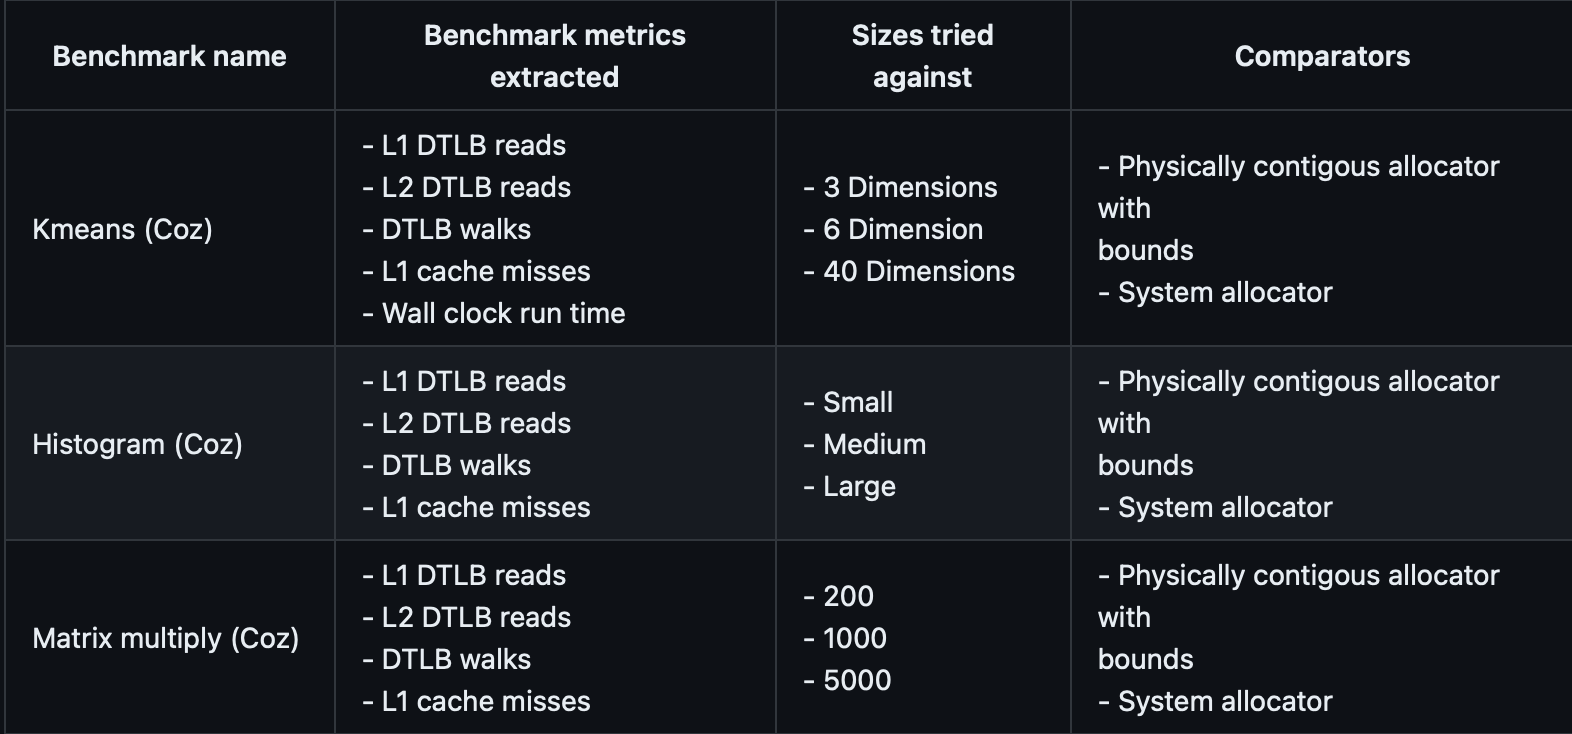
\includegraphics[width=0.8\textwidth]{diagrams/expirement-runs.png}
  \caption{C programs evaluated}
\end{figure}

\subsection{DTLB L1 reads}
% L1 TLB graphs
\begin{figure}
  \begin{subfigure}{\linewidth}
  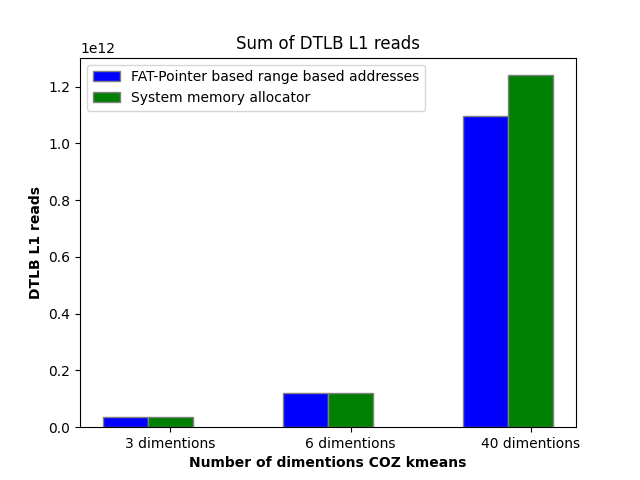
\includegraphics[width=.5\linewidth]{l1-tlb-kmeans.png}\hfill
  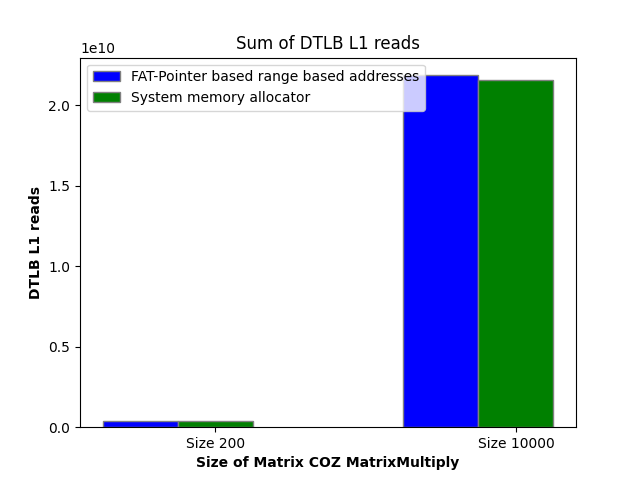
\includegraphics[width=.5\linewidth]{l1-tlb-matrixmultiply.png}\hfill
  \includegraphics[width=.5\linewidth]{l1-tlb-histogram.png}
\end{subfigure}
\caption{DTLB L1 reads}
\label{TLBl1}
\end{figure}
The Graphs above\ref{fig:TLBl1} represent the DTLB L1 reads which is a Performance counter from the ARM specs. 
The counter increments for every Memory-read or Memory-write operation that necessitates an 
access to the Level 1 data or unified Translation Lookaside Buffer (TLB). 
Each access to a TLB entry is counted including multiple accesses caused by single instructions.

\subsection{DTLB L2 reads}
% L2 TLB graphs
\begin{figure}
  \begin{subfigure}{\linewidth}
    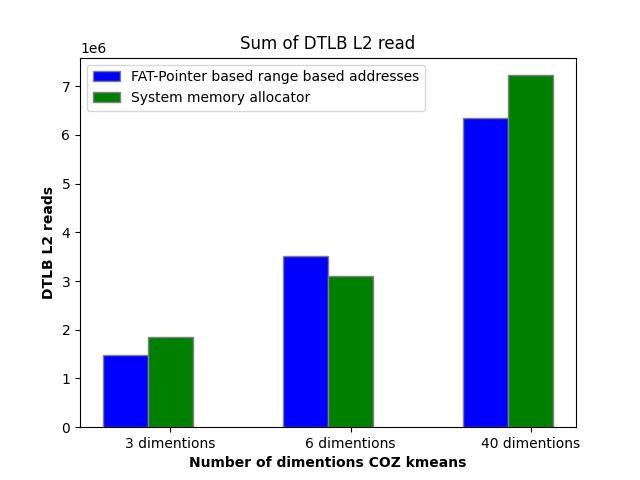
\includegraphics[width=.5\linewidth]{l2-tlb-kmeans.png}\hfill
    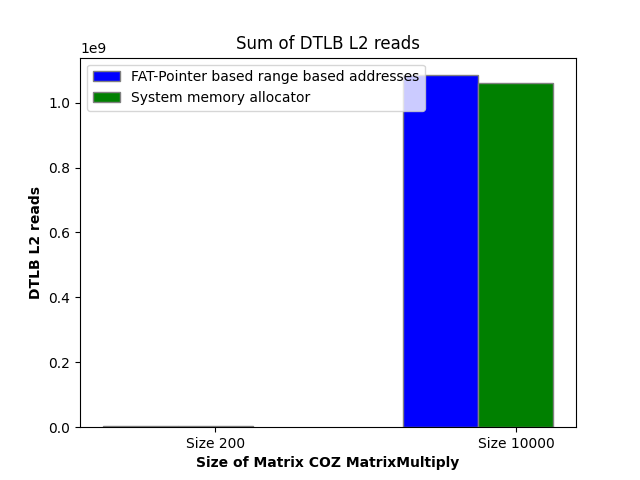
\includegraphics[width=.5\linewidth]{l2-tlb-matrixmultiply.png}\hfill
    \includegraphics[width=.5\linewidth]{l2-tlb-histogram.png}
\end{subfigure}
\caption{DTLB L2 reads}
\label{TLBl2}
\end{figure}
Similar to how L1 TLB reads are counted, DTLB L2\ref{fig:TLBl2} counts every read operation that accesses the 
Level 2 data or unified TLB. Each time there is a read to an entry in the Level 2 TLB, 
it is counted by the ARM performance counter. 

% DTLB walks
% - Explain how the stat is calculated 
% - Fix older paragraphs 

\subsection{DTLB walks}
\begin{figure}
  \begin{subfigure}{\linewidth}
    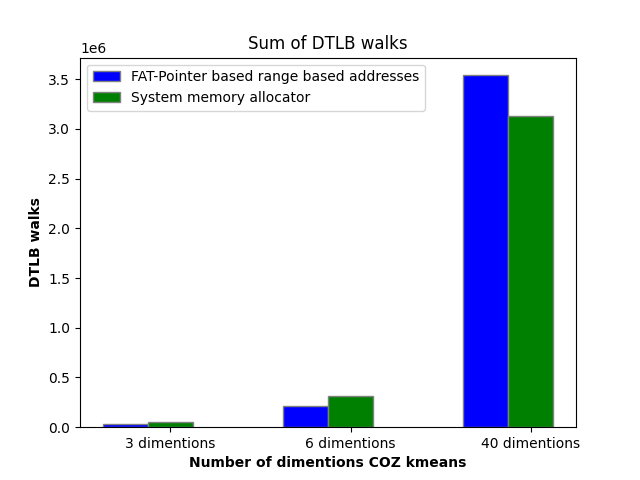
\includegraphics[width=.5\linewidth]{tlb-walk-kmeans.png}\hfill
    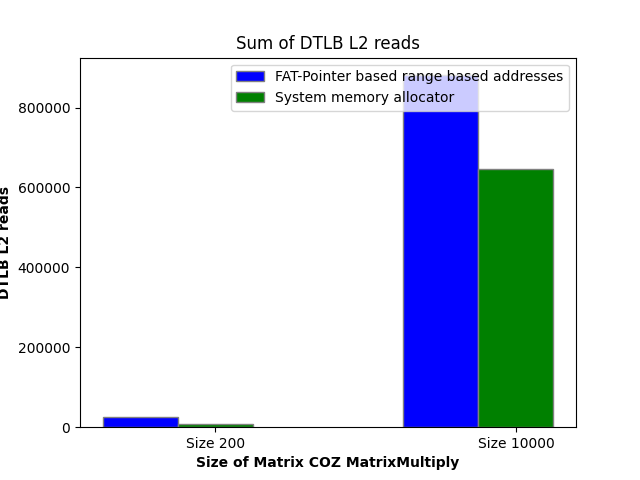
\includegraphics[width=.5\linewidth]{tlb-walk-matrixmultiply.png}\hfill
    \includegraphics[width=.5\linewidth]{tlb-walk-histogram.png}
\end{subfigure}
\caption{DTLB Walks}
\label{TLBWalk}
\end{figure}

The DTLB walk\ref{fig:TLBWalk} counter counts each Memory-read operation or Memory-write operation that causes a 
TLB access to at least the Level 2 data or unified TLB.
Each access to a TLB entry is counted including refills 
of Level 1 TLBs.

% L1 cache miss
\subsection{L1 cache miss}
\begin{figure}
  \begin{subfigure}{\linewidth}
    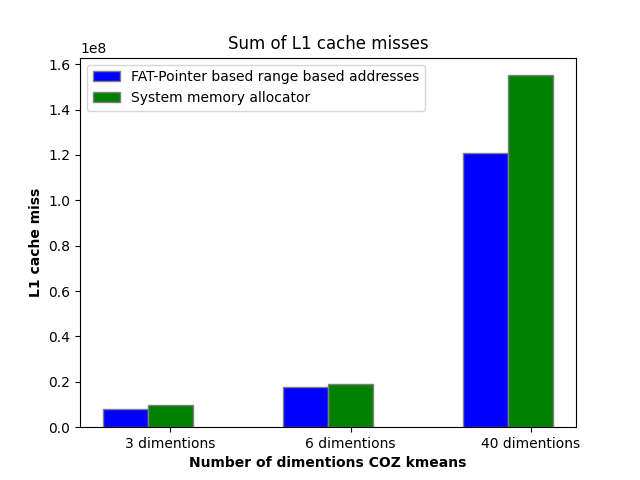
\includegraphics[width=.5\linewidth]{l1-miss-kmeans.png}\hfill
    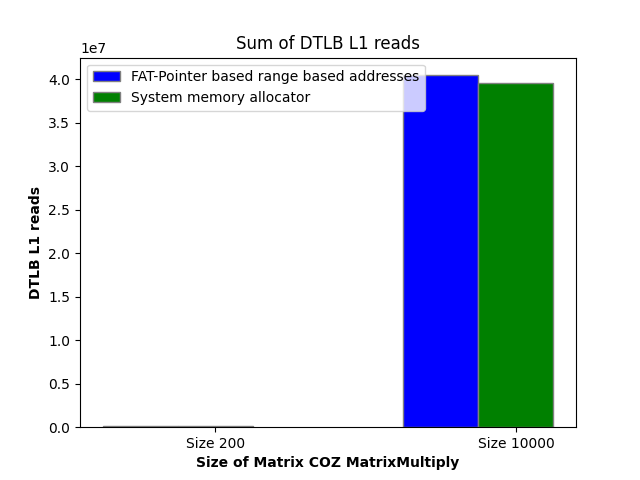
\includegraphics[width=.5\linewidth]{l1-miss-matrixmultiply.png}\hfill
    \includegraphics[width=.5\linewidth]{l1-miss-histogram.png}
\end{subfigure}
\caption{L1 Cache misses}
\label{L1CacheMiss}
\end{figure}
L1 cache miss\ref{fig:L1CacheMiss} counter counts each Memory-read operation to the Level 1 data or unified cache counted by L1 cache miss counter that incurs additional latency because it returns data from outside of the Level 1 data or unified cache of this PE.
The event indicates to software that the access missed in the Level 1 data or unified cache and might have a significant performance impact due to the additional latency compared to the latency of an access that hits in the Level 1 data or unified cache.
\newline
% • Accesses where the additional latency is unlikely to be significantly performance-impacting. For example, if the access hits in another cache in the same local cluster, and the additional latency is small when compared to a miss in all Level 1 caches that the access looks up in and results in an access being made to a Level 2 cache or elsewhere beyond the Level 1 data or unified cache.
% • A miss that does not cause a new cache refill but is satisfied from a previous miss.

% The Benchmark results indicates bugs in the sample FAT-Pointer based range address prototype
% memory allocator. This is an ongoing evaluation and results provided above are a snapshot of the
% latest results. For the use case of the L2 TLB reads for the FAT-Pointer based range address prototype
% show that there are reads. This means that there are bugs in the implementation since all reads should 
% be through the L1TLB since for the program memory is pre-allocated as single physically contgious page. 

\section{Analysis}

The benchmark results indicate the presence of bugs in the sample FAT-Pointer based range address prototype memory allocator. This evaluation is ongoing, and the 
results provided here\ref{fig:TLBl1}\ref{fig:TLBl2}\ref{fig:TLBWalk}\ref{fig:L1CacheMiss} represent a snapshot of the latest findings. Specifically, for the use case of Level 2 Translation Lookaside Buffer (L2 TLB) reads, 
the FAT-Pointer based range address prototype shows occurrences of reads from the L2 TLB. This indicates the presence of implementation bugs, 
as all reads should be managed through the Level 1 Translation Lookaside Buffer (L1 TLB), given that the program memory is pre-allocated as a single 
physically contiguous page.
\newline

In a correctly functioning system, the L1 TLB should handle all memory accesses, ensuring efficient translation and minimizing latency. 
The detection of L2 TLB reads suggests that there are flaws in the current implementation, potentially in the memory allocation or 
address translation mechanisms. These bugs need to be addressed to achieve the intended performance and correctness of the 
FAT-Pointer based range address prototype memory allocator. Further investigation and debugging are required to 
identify the exact causes and rectify these issues to ensure that all memory accesses are correctly routed 
through the L1 TLB as designed.
\newline

The ContigMalloc function in CheriBSD is designed to allocate contiguous blocks of physical memory. In theory, this should result in a single large block of memory 
that is efficiently handled by the L1 cache, reducing cache misses and improving performance. However, the observed behavior suggests otherwise.
\newline

A slab allocator divides memory into small, fixed-size chunks or "slabs" for allocation. While this can be efficient for managing 
objects of uniform size, it can lead to increased cache misses if objects are not optimally aligned or if there is fragmentation. 
The slab allocation pattern can cause data to be scattered across different cache lines, leading to inefficient cache usage.
\newline

In the k-means C program, which involves intensive computation and frequent memory accesses, L1 cache efficiency is 
crucial for performance. The presence of significant L1 cache misses indicates that the memory allocation is not as 
contiguous as expected. Instead, it suggests that the memory may be fragmented or scattered, similar to what happens with a slab allocator.
\newline

Given the behavior of ContigMalloc and the observed cache performance, it is speculated that ContigMalloc may be 
functioning in a manner similar to a slab allocator under the hood. This could involve internal mechanisms that 
break down the large contiguous allocation request into smaller chunks or slabs for management, inadvertently 
causing the observed L1 cache misses.
\newline

The deviation from truly contiguous allocation impacts the performance of programs like k-means, which rely on efficient 
memory access patterns. L1 cache misses can significantly slow down computation, as accessing data from higher-level 
caches or main memory introduces additional latency. To confirm this hypothesis, further investigation is needed. 
This includes analyzing the internal implementation of ContigMalloc to understand its allocation strategy, 
profiling the memory allocation patterns and cache usage in detail, and conducting controlled experiments 
to compare the behavior of ContigMalloc with known slab allocators.
\newline

If the hypothesis is confirmed, potential solutions could involve modifying ContigMalloc to ensure truly contiguous 
physical memory allocation, implementing custom memory allocators tailored to the specific needs of high-performance 
applications like k-means, and optimizing the existing allocation strategy to minimize fragmentation and improve cache 
utilization. In summary, while ContigMalloc is intended to provide contiguous memory allocation, its current behavior 
suggests a resemblance to slab allocation, leading to suboptimal L1 cache performance in the k-means C program. 
This calls for a deeper dive into the allocator's implementation and strategic adjustments to achieve the 
desired memory access efficiency.

\chapter{Future work}
% The future plan is to transition from the current experiment, which involves working on the ARM architecture on the ARM Morello board. 
% The current limitation is that all memory reads must go through the TLB for translations. The future plan involves storing 
% the offset directly on the pointer and using the bounds in CHERI to enable block-based allocator behavior. This phase of the 
% experiment is intended to be conducted on the RISC-V implementation of CHERI, known as Tooba. 

% In the RISC-V implementation, the hardware Verilog design will be modified to allow bypassing the TLB. Once this concept is 
% integrated into the RISC-V Verilog implementation, the OS layer will be changed to a single-address-space operating system, 
% where there is no distinction between user space and kernel space. In this implementation, the kernel allocator will be the 
% same as the user space allocator since both can utilize a single contiguous chunk of memory.
The current experimental setup on the ARM Morello board is constrained by the requirement that all memory reads must 
pass through the Translation Lookaside Buffer (TLB) for address translation. This necessitates frequent TLB lookups, potentially 
leading to performance bottlenecks. The planned future work aims to address this by leveraging CHERI 
(Capability Hardware Enhanced RISC Instructions) extensions on the RISC-V architecture, specifically using the 
Tooba implementation.

\subsubsection{Storing Offsets Directly on Pointers}
In the current ARM Morello setup, address translations rely on the TLB.
The future approach on RISC-V Tooba involves storing the offset directly within the pointer. This is possible due to CHERI's capability model, which supports fine-grained memory protection and can encode bounds within pointers.
Utilizing Bounds in CHERI for Block-Based Allocation:

CHERI capabilities allow pointers to carry metadata about memory bounds, providing hardware-enforced memory safety.
By encoding the offset and bounds within the pointer, the system can directly access memory without needing intermediate translations via the TLB.
This enables the implementation of a block-based allocator that can efficiently manage memory allocations and deallocations within defined bounds.
Bypassing the TLB in RISC-V Tooba.
\subsubsection{Hardware Modifications}:
The Verilog design of the RISC-V processor will be modified to allow certain memory operations to bypass the TLB. This means that when a pointer with encoded offset and bounds is used, the system can directly compute the physical address from the capability information.
This modification reduces the dependency on the TLB, decreasing latency and improving performance, especially for frequent memory operations.
Transition to a Single-Address-Space Operating System (SASOS).
\subsubsection{Concept of SASOS}:
In traditional operating systems, there is a clear separation between user space and kernel space. This separation is enforced by memory protection mechanisms and address translation through the TLB.
In a Single-Address-Space Operating System, this distinction is removed. Both user applications and the kernel share the same contiguous address space.
\subsubsection{Advantages of SASOS with CHERI}:
\begin{itemize}
  \item Simplified Memory Management : Without the need to switch between user and kernel spaces, memory management becomes simpler and more efficient.
The kernel allocator can be the same as the user space allocator, operating on a single, contiguous chunk of memory.
  \item Unified Allocator: The unified memory allocator can efficiently manage memory for both kernel and user applications, leveraging CHERI's capability-based protection to prevent unauthorized access.
This reduces overhead and potential fragmentation issues associated with maintaining separate memory spaces.
\end{itemize}
% %!TEX root = ../thesis.tex
%*******************************************************************************
%*********************************** Research Questions *****************************
%*******************************************************************************

\chapter{Research Questions}  %Title of the Research Questions

The following section talks about research questions: 

\begin{itemize}
    \item Which areas can Unikernels provide performance gains for TAG based architectures in comparison to the same implementation built using a monolithic OS? 
    \item Does using Enclaves inside Unikernels provide a isolation mechanism within Unikernels, maintain lightweightness characterestics, and 
    what would be the performance differnence between using Intel SGX and a open source implementation such as Timber V?
    \item Due to lesser depencies in Unikernels does that mean lesser TAG policies are required for the appication ? 
    \item Can Unikernel provide sufficient performance in such a way that a dedicated processor is not required for processing TAGS ?   
    \item Does Unikernels with TAGS provide a secure and elastic environment ? 

    % New ones 
    \item Using TAG standard memory with interleaving for speeding up types for dynamic languages and execution of parallelization on Mult-kernels with each core 
          running a Uni-kernel.
\end{itemize}
% ]%!TEX root = ../thesis.tex
%*******************************************************************************
%*********************************** Literature Review *****************************
%*******************************************************************************

\chapter{Literature Review}  %Title of the Literature Review

\ifpdf
    \graphicspath{{LiteratureReview/Figs/Raster/}{LiteratureReview/Figs/PDF/}{LiteratureReview/Figs/}}
\else
    \graphicspath{{LiteratureReview/Figs/}{LiteratureReview/Figs/}}
\fi

%********************************** %Introduction for literature review **************************************

The literature review is split into 3 sections. The first section talks about the papers surveyed 
for Unikernels and the 2nd section talks about papers surveyed for TAG based architectures and 
the third sections talks about the possible incentives of combining them both which helps 
answer the research questions stated (TODO: Add reference to research question section). 

\section[Unikernels]{Unikernels Survey}
The following section is the Uni-kernel Survey which starts 
with the Introduction of Unikernels, Types of Uni-kernels, 
Various Uni-kernels implementations and analysis 
of the various Uni-kernel implementations. 

\subsection{Introduction to Unikernels}
Unikernel is a relatively new concept that was first introduced around 2013 by Anil Madhavapeddy in a 
paper titled "Unikernels: Library Operating Systems for the Cloud" \cite{FirstUnikernelPaper}. Unikernels 
is defined as "Unikernels are specialized, single-address-space machine images constructed by using library 
operating systems." \cite{UnikernelDefinition}. Specialized indicates that an Unikernel holds a single application.
Single address indicates that Unikernels does not have separation between the user and kernel address 
space. 

\begin{figure}[htbp!] 
  \centering    
  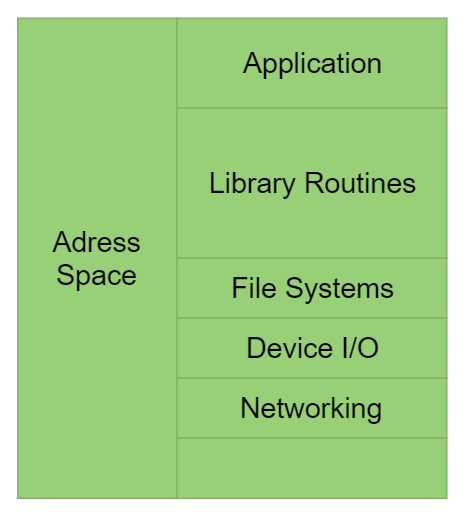
\includegraphics[width=0.2\textwidth]{unikernel_application_stack}
  \caption[Unikernel]{Unikernel application stack \cite{UnikernelSurvey}}
  \label{fig:unikernel_application_stack}
  \end{figure}

  \begin{figure}[htbp!] 
    \centering    
    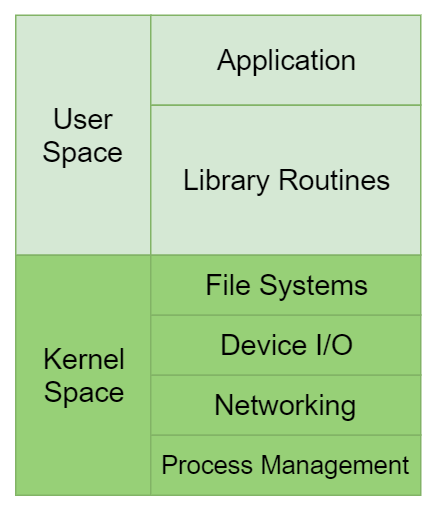
\includegraphics[width=0.2\textwidth]{normal_application_stack}
    \caption[Normal]{Normal application stack \cite{UnikernelSurvey}}
    \label{fig:normal_application_stack}
    \end{figure}

\subsubsection{Library Operating Systems}
Library\cite{LibraryOS} operating system is an method of constructing an operating system where the kernel modules  
required by an application is executed in the same address space as the application. The original goal 
of Library operating systems was to improve performance by enabling applications to manage resources according to 
their own needs, thereby allowing a high level of customizability. One of the major drawbacks for 
Library OS was support for various device drivers written for specific hardware. 

Nowadays, however, virtualization already provides an abstraction of the underlying hardware by exposing 
virtualized hardware drivers. This allows library OS implementations to support the generic virtual driver 
as opposed to attempting to support various hardware drivers.

% Definition of Unikernels 
% Primary Software Stacks the Unikernel is supported for 
% Diagram of Unikernels 


\subsection{Types of Unikernels}
% Library OS 
% Binary Compatible Uni-kernels 
\subsubsection{Clean slate (Specialized and purpose-built unikernels)}
Designed to utilize all the modern features of software and hardware, without worrying about backward
compatibility. They are not POSIX-compliant. 
\begin{itemize}
  \item Halvm (TODO survey)
  \item MirageOS (TODO survey)
\end{itemize}

\subsubsection{Legacy (Generalized "fat" unikernels)}
Designed to run unmodified applications in an Unikernel, 
which make them bulky in comparison to the clean slate approach. 
Designed to be POSIX compliant. The following below 
are the ones surveyed in the following paper: 
\begin{itemize}
  \item Unikraft
  \item OSv 
  \item HermitCore 
  \item RKOS
  \item Azelea
  \item IncludeOS 
  \item ClickOS
  \item NanoOS
\end{itemize}
%
% 4. Figures for all implementations 
% 5. References for all implementations 
% 6. Table analyses for all implementations 
% 7. More on Hermit core (Phrase research questions based on Hermit core)
%
\subsection{Implementations}

\subsubsection{Unikraft \cite{Unikraft}}
Unikraft is a uni-kernel implementation that claims to be 
a micro library OS. \emph{The major features of Unikraft is:}
\begin{itemize}
  \item Single address space: Intended to target single applications.
  \item Fully modular system: All drivers and platform libraries can be easily removed.
  \item Single protection level: No kernel and user space separation to avoid costly context switching.
  \item Static linking: Compiler features such as dead code elimination and link time optimization supported. 
  \item POSIX support: Support for legacy applications while still allowing for specialization. 
  \item Platform abstraction: The ability to run on different Hypervisors/VMs. 
\end{itemize}
\emph{To reach for the principal of modularity. Unikraft consists of 2 major components:}
\begin{itemize}
  \item Micro libraries: Micro-libraries are software components 
  which implement one of the core Unikraft APIs.
  \item Build system: The build system
  then compiles all of the micro-libraries, links them,
  and produces one binary per selected platform.
\end{itemize}
\emph{In terms of performance the following was evaluated in Unikraft:}
\begin{itemize}
  \item Resource Efficiency (Smaller is Better): Overall, the total VM boot time is dominated by the VMM,
  with Solo5 and Firecracker being the fastest (3ms), QEMU
  microVM at around 10ms and QEMU the slowest at around
  40ms.
  \item Filesystem Performance: Unikraft
  achieves lower read latency and lower write latency with
  different block sizes and are considerably better than ones
  from the Linux VM.
  \item Application Throughput: Unikraft is around 30\%-80\% faster than running the same app
  in a container, and 70\%-170\% faster than the same app running 
  in a Linux VM. Surprisingly, Unikraft is also 10\%-60\%
  faster than Native Linux in both cases.
  \item Performance of Automatically Ported Apps: The results
  show that the automatically ported app is only 1.5\% slower
  than the manually ported version, and even slightly faster
  than Linux bare-metal.
\end{itemize}

\begin{figure}[htbp!] 
  \centering    
  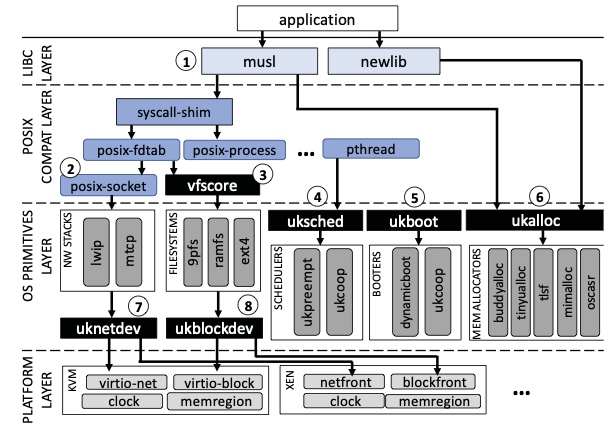
\includegraphics[width=0.6\textwidth]{UnikraftStack}
  \caption[Unikraft]{Unikraft application stack \cite{Unikraft}}
  \label{fig:UnikraftStack}
  \end{figure}
  % source https://dl.acm.org/doi/pdf/10.1145/3447786.3456248

\subsubsection{OSv}
OSv\cite{OSvPaper} is an Unikernel that runs existing Linux cloud applications on various hypervisors 
and machine architectures. OSv runs on 64-bit x86 and
ARM architectures and supports KVM/Qemu, VMware, Xen and VirtualBox 
hypervisors.OSv demonstrates up to 25\% increase in throughput and 47\% 
decrease in latency. 
By using non-POSIX network APIs,
it can further improve performance and demonstrate a
290\% increase in Memcached throughput.
OSv is designed as a drop-in replacement for applications that use a
supported subset of the Linux application binary interface (ABI).
\emph{The following below is the design of OSv:}
\begin{itemize}
  \item Memory Management: OSv uses virtual memory like
  general purpose OSs.OSv supports demand paging and memory mapping
  via the mmap API.
  \item No Spinlocks: The mutex implementation is based on a lock-free design 
  by Gidenstam \& Papatriantafilou \cite{LockFree}, which protects
  the mutex's internal data structures with atomic operations in a lock-free fashion.
  \item Network Channels: In OSv almost all packet processing is performed in an application thread. 
  Upon packet received, a simple classifier associates it with a channel, which is a single producer/single
  consumer queue for transferring packets to the application thread.
\end{itemize}

\begin{figure}[htbp!] 
  \centering    
  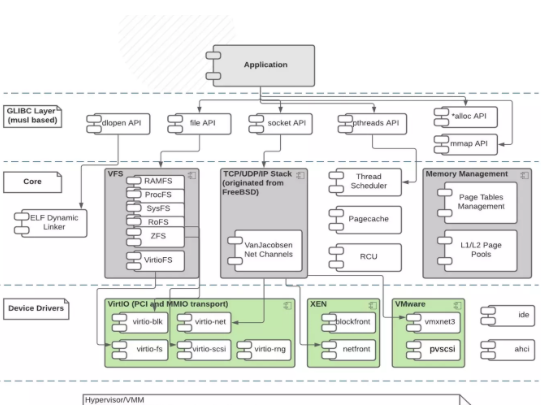
\includegraphics[width=0.7\textwidth]{OSvStack}
  \caption[OSv]{OSv application stack \cite{OSvDiagram}}
  \label{fig:OSv}
  \end{figure}
  % source https://www.slideshare.net/ScyllaDB/osv-unikernel-optimizing-guest-os-to-run-stateless-and-serverless-apps-in-the-cloud



\subsubsection{HermitCore}
HermitCore\cite{HermitCore} is an Unikernel implementation designed for HPC. The kernel extends the
multi-kernel approach with the advantages of a Unikernel.The focus of HermitCore is 
the mapping of the hardware to
the software structure rather than full support of the Linux
API.In a HermitCore system, each NUMA node runs its own HermitCore instance managing all its resources.
\emph{The aims for Hermit core are the following:}
\begin{itemize}
  \item Reduction of OS noise.
  \item Predictable runtimes.
  \item Maintainability, extensibility, and flexibility.
  \item Abstraction of hardware details.
  \item Support for common HPC programming models (e. g.,
  OpenMP, MPI).
  \item Simple integration into existing software stacks of
  compute centers.
\end{itemize}
\emph{Benchmarks conducted:}
\begin{itemize}
  \item Operating System Micro-Benchmarks.
  \item Hourglass Benchmark (For OS Noise).
  \item Inter-kernel Communication Benchmark.
  \item OpenMP Micro-Benchmarks.
\end{itemize}
\emph{The following are derived projects from the hermit-core project:}
\begin{itemize}
  \item HermitTux \cite{Hermitux} : It is a linux binary compatible Unikernel that can run native linux executables. 
  \item RustyHermit \cite{RustyHermit}: Implementation of the Hermit core Unikernel in Rust. 
  \item Lib-hermitMPK \cite{HermitMPK} : Providing support for IntelMPK for RustyHermit to isolate the unsafe parts of the kernel and 
  application with proven performance similar RustyHermit without the memory protection.
\end{itemize}
% \begin{itemize}
%   \item HermitTux : It is a linux binary compatible Unikernel that can run native linux executables. 
%   \item RustyHermit : Implementation of the Hermit core Unikernel in Rust. 
%   \item Lib-hermitMPK : Providing support for IntelMPK for RustyHermit to isolate the unsafe parts of the kernel and isolate 
%   the application with a similar performance of RustyHermit without the memory protection.
% \end{itemize}

\begin{figure}[htbp!] 
  \centering    
  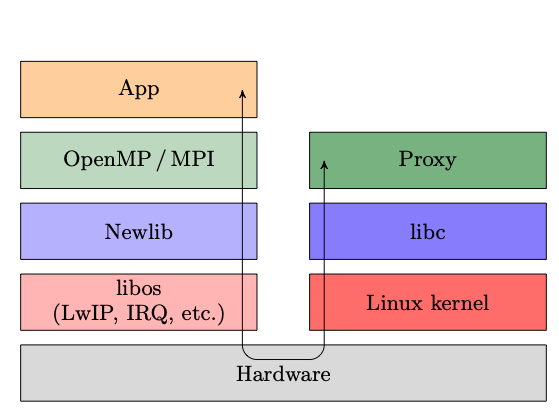
\includegraphics[width=0.5\textwidth]{HermitCoreStack}
  \caption[HermitCore]{HermitCore Software stack \cite{HermitCore}}
  \label{fig:HermitCoreStack}
  \end{figure}
  % source https://dl.acm.org/doi/pdf/10.1145/2931088.2931093

  \begin{figure}[htbp!] 
    \centering    
    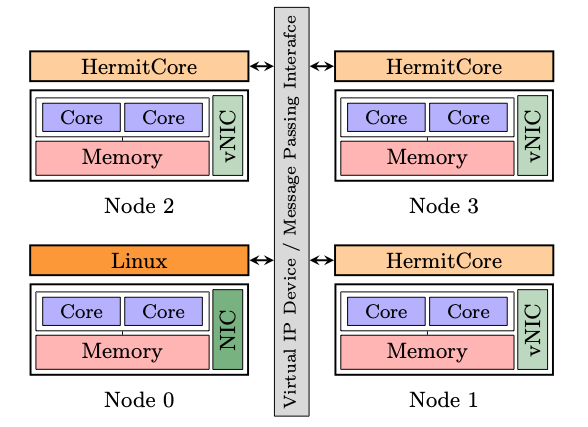
\includegraphics[width=0.8\textwidth]{NumaHermitCore}
    \caption[HermitCore]{A NUMA system with one satellite kernel per NUMA node \cite{HermitCore}}
    \label{fig:HermitCoreStack}
    \end{figure}
    % source https://dl.acm.org/doi/pdf/10.1145/2931088.2931093



\subsubsection{RKOS}
% source: https://media.taricorp.net/rkos.pdf
RKOS\cite{RKOS} is an unikernel implemented in Rust which
offers safety guarantees comparable to implementations which depend on complex runtime
libraries while being capable of providing predictable application performance demanded
by real-time applications in a relatively simple implementation. 
\emph{Design decisions for RKOS are as follows:}
\begin{itemize}
  \item Mutual trust between components allows a shared, uniform address space.
  \item Virtualized runtime environments have uniform hardware configuration.
\end{itemize}
\emph{Performance Evaluations conducted:}
\begin{itemize}
  \item Run time memory footprint 
  \item Binary size 
\end{itemize}

\subsubsection{ClickOS}
ClickOS\cite{ClickOS} is an unikernel optimized for middleboxes that runs exclusively on
the Xen hypervisor with small virtual machine memory footprint overhead
(5 MB), fast boot times (under 30 milliseconds), and high performance
networking capabilities.ClickOS adds only a 45 microsecond delay per
packet. When compared to a general purpose Linux also running on Xen,
ClickOS network throughput is up to 1.5x times higher for MTU-sized packets
and as much as 13.6x times higher for minimum-sized packets. 

\begin{figure}[htbp!] 
  \centering    
  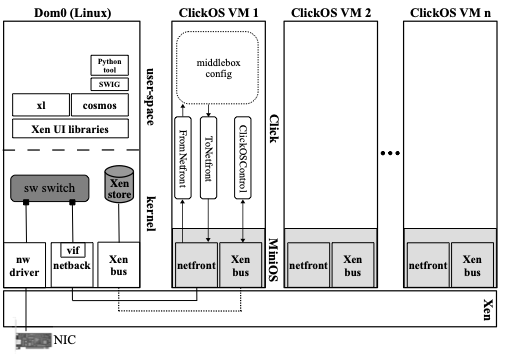
\includegraphics[width=0.6\textwidth]{ClickOSStack}
  \caption[ClickOS]{ClickOS architecture \cite{ClickOS}}
  \label{fig:ClickOSStack}
  \end{figure}
  % source https://www.usenix.org/system/files/conference/nsdi14/nsdi14-paper-martins.pdf

\subsubsection{NanoOS \cite{NanoOS}}
Nanos is a Unikernel implementation designed to run micro services on the 
Cloud, it runs on top of a Qemu Hypervisor and has it's own Orchestrator 
written in Go called OPS. 
Nanos employs various forms of security measures found in other general purpose operating systems including ASLR and respects page protections 
that the compilers produce.

\emph{ASLR:}

\begin{itemize}
  \item Stack Randomization
  \item Heap Randomization
  \item Library Randomization
  \item Binary Randomization
\end{itemize}

\emph{Page Protections:}

\begin{itemize}
  \item Stack Execution off by Default
  \item Heap Execution off by Default
  \item Null Page is Not Mapped
  \item Rodata no execute
  \item Text no write
\end{itemize}

\begin{itemize}
  \item SMEP
  \item UMIP
\end{itemize}

\emph{Performance Evaluations conducted:}
\begin{itemize}
  \item Bootup Times.
  \item Requests per second.
\end{itemize}

\subsubsection{IncludeOS}
IncludeOS\cite{IncludeOS} is a single tasking library operating system for 
cloud services which is written from scratch in C++. Key features include:
extremely small disk and memory footprint, efficient asynchronous I/O, 
OS-library where only what your service needs gets included.
In the test case the bootable disk image consisting
of a simple DNS server with OS included is shown
to require only 158 kb of disk space and to require
5-20\% less CPU-time.
\emph{The contributions of IncludeOS are:}
\begin{itemize}
  \item Extreme resource efficiency and footprint.
  \item Efficient deployment process.
  \item Virtualization platform independence.
\end{itemize}
\emph{The proposed benefits of IncludeOS  in comparison to Linux Kernels are:}
\begin{itemize}
  \item Extremely small disk and memory footprint.
  \item No host or software dependencies, other than
  virtual x86 hardware, and standard virtio for
  networking
  \item No system call overhead (The OS and the
  services are in the same binary, and the system calls
  are simple function calls(i.e without passing any
  memory protection barriers)).
  \item Reduced number of VMs exits by keeping the
  number of protected instructions very low.
\end{itemize}

\emph{Performance Evaluations conducted:}
\begin{itemize}
  \item Bootup times 
  \item Memory performance (i.e The Stream Benchmark)
\end{itemize}

\subsubsection{Azelea}
Azalea\cite{Azelea} is a multi-kernel OS, which consists of Unikernels and a full kernel. Azelea Unikernel provides scalability and parallel performance. 
The full kernel provides compatibility with POSIX APIs that the Unikernel cannot handle. The Full kernel is combined with the Unikernel for 
side by side partitioning. \emph{The Azelea Unikernel is a library OS which consists of the following:}
\begin{itemize}
  \item Kernel Functions 
  \item Run time libraries 
  \item Application 
\end{itemize}
A server can run multiple Azelea-unikernels with the number of cores and memory allocated. The Linux install which is a part of 
the server acts as a driver and that loads each Unikernel or supports communication between other nodes. 
\emph{The contributions of Azelea Uni-kernels are:}
\begin{itemize}
  \item Lightweight kernel.
  \item Compatibility with legacy application (i.e Support for statically build Linux binaries).
  \item I/O offloading (i.e FWK(Full weight kernel) handles all the I/O offloading so that applications can be executed without any interference). 
\end{itemize}

\emph{Performance Evaluations conducted:}
\begin{itemize}
  \item OS Noise (FTQ, FWQ, Hour Glass) \cite{AzeleaOSNoise}
  \item IO offload acceleration \cite{AzeleaIOAccerleration}
\end{itemize}

\begin{figure}[htbp!] 
  \centering    
  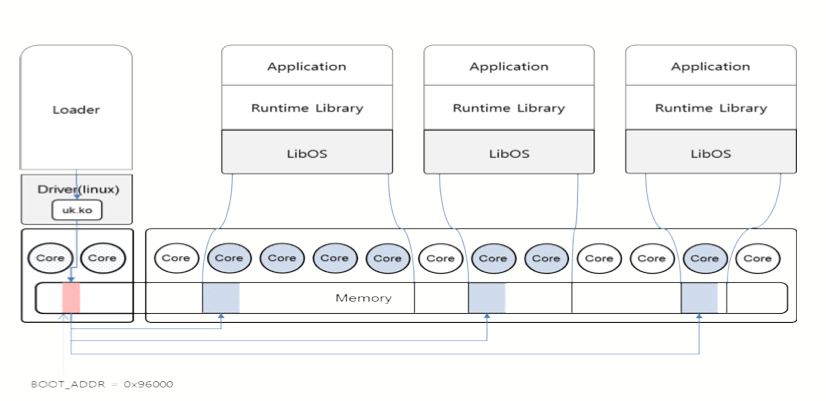
\includegraphics[width=0.6\textwidth]{AzeleaKNL}
  \caption[Azelea]{Azelea-unikernel in a single KNL \cite{Azelea}}
  \label{fig:AzeleaKNL}
  \end{figure}
  % source https://ieeexplore.ieee.org/stamp/stamp.jsp?tp=&arnumber=8539634

\subsubsection{HaLVM}
HaLVM(Haskell Lightweight Virtual machine) is an unikernel implementation based on Xen hypervisor (i.e type 1 hypervisor). 
HaLVM is implemented using Haskell. HaLVM is suitable for small, single-use and
low-dependence programs. There was only 1 published work was a paper on analyzing 
parallel programs model for HaLVM\cite{HaLVM}. 

% \emph{Performance Evaluations conducted(parallel model):}
% \begin{itemize}
%   \item Eval monad
%   \item forkIO
%   \item forkOS
%   \item Cloud Haskell
%   \item IVC
% \end{itemize}

\begin{figure}[htbp!] 
  \centering    
  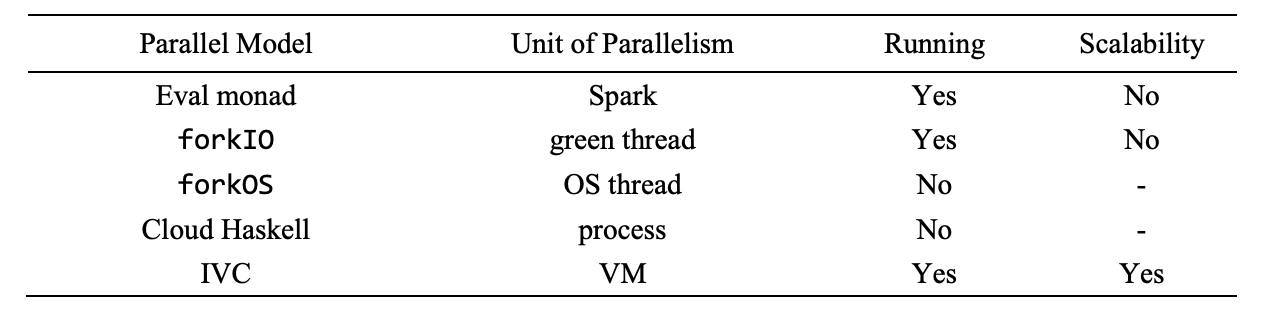
\includegraphics[width=0.8\textwidth]{halvm-execution}
  \caption[halvm-execution]{Performance Evaluations conducted(parallel model) \cite{HaLVM}}
  \label{fig:HaLVM}
  \end{figure}

\begin{figure}[htbp!] 
  \centering    
  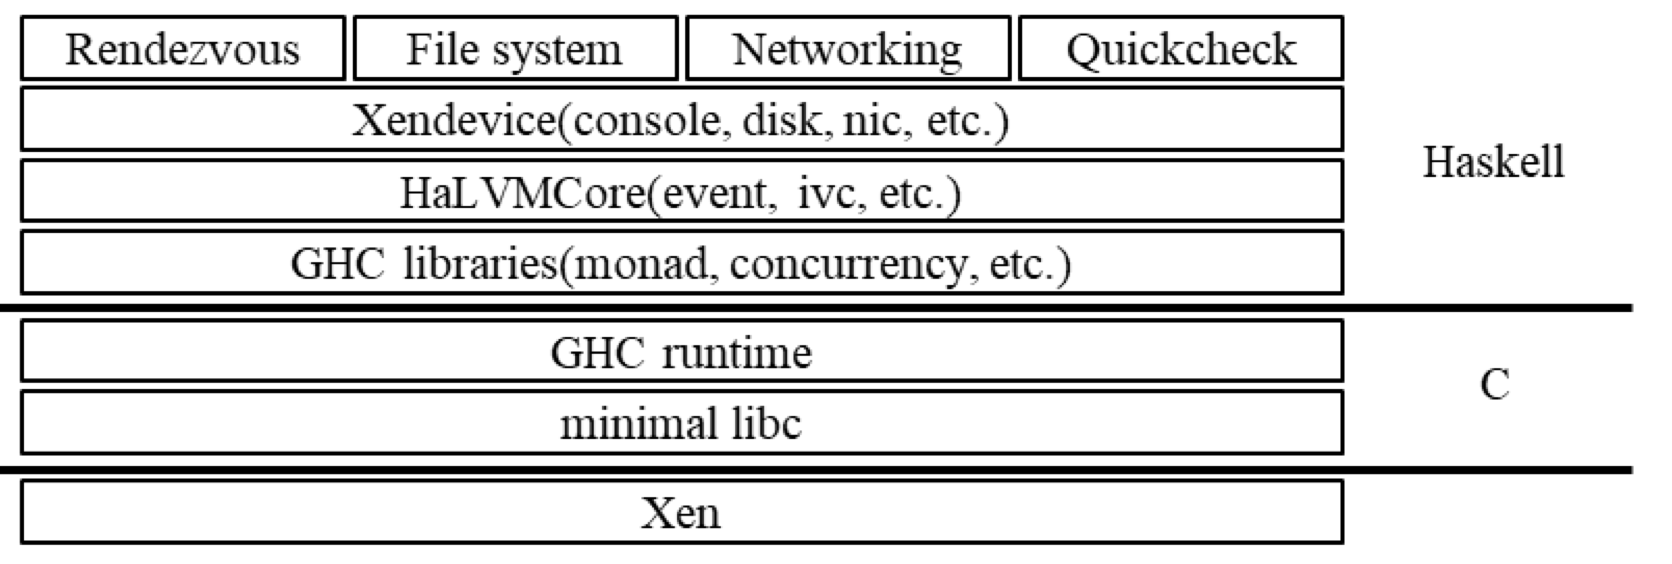
\includegraphics[width=0.6\textwidth]{halvm}
  \caption[HaLVM]{HaLVM architecture \cite{HaLVM}}
  \label{fig:HaLVM}
  \end{figure}

  \subsubsection{Mirage}
  Mirage\cite{mirage} produces an Unikernel by compiling and 
  linking OCaml to an Xen VM image. The objective 
  was to combine static type-safety with a single
  address-space layout. Using Mirage it is possible 
  to use libraries such as networking, storage and concurrency
  that works under unix during development, when compiled 
  to production becomes operating system drivers. 

  \emph{Mirage takes advantage of Ocaml for the following reasons:}
  \begin{itemize}
    \item Static type checking
    \item Automatic memory management
    \item Modules
    \item Metaprogramming
  \end{itemize}

  \emph{Performance Evaluations conducted:}
  \begin{itemize}
    \item Boot time.
    \item Thread performance.
    \item Throughput.
    \item Sessions per for a sample dynamic web application.
  \end{itemize}
  
  \begin{figure}[htbp!] 
    \centering    
    \includegraphics[width=0.6\textwidth]{Mirage}
    \caption[Mirage]{Azelea-unikernel in a single KNL \cite{Azelea}}
    \label{fig:Mirage}
    \end{figure}

\subsection{Unikernel analysis}
The following section consists of analysis of the Uni-kernels 
implementations surveyed in the current literature. The 
analyses is based on: 
\begin{itemize}
\item Best suitable implementations for various platforms supported ? 
% \item Best suitable for various architectures ?
% \item Best implementation in terms of performance ?
\item How do each of them handle parallel applications ?
% \item Best tools with the most concrete evaluation ? 
\end{itemize}


% \begin{table}[]
%   \resizebox{\columnwidth}{!}{%
%   \begin{tabular}{@{}|l|l|l|l|@{}}
%   \toprule
%   \textit{\textbf{Unikernel}} & \textit{\textbf{Languages supported}}                                                                   & \textit{\textbf{Targets}}                                                                            & \textbf{Performance evaluation}                                                                                                                                                                                                                   \\ \midrule
%   \textit{Unikraft\cite{Unikraft}}           & \textit{C, C++, Rust, Go, Python}                                                                       & \textit{\begin{tabular}[c]{@{}l@{}}KVM, Xen, Linux Userspace, Solo5, \\ VMware, HyperV\end{tabular}} & \begin{tabular}[c]{@{}l@{}}- Resource \\   Efficiency \\ - Filesystem \\   Performance \\ - Application \\   throughput. \\ - Performance of \\   Automatically ported \\   apps.\end{tabular}                                                    \\ \midrule
%   OSv\cite{OSvPaper}                         & Java, C, C++, Node, Ruby, Go                                                                            & Virtual Box, EXSi, KVM and HyperV.                                                                   &                                                                                                                                                                                                                                                   \\ \midrule
%   NanoOS\cite{NanoOS}                     & \begin{tabular}[c]{@{}l@{}}C, C++, Go, Java, Node js, Python, \\ Rust, Rust, Ruby, and PHP\end{tabular} & \begin{tabular}[c]{@{}l@{}}KVM, XEN,ESXi and \\ Hyper V\end{tabular}                                 & \begin{tabular}[c]{@{}l@{}}- Boot Up \\    times \\ - Request \\   per second\end{tabular}                                                                                                                                                        \\ \midrule
%   HermitCore\cite{HermitCore}                  & Rust, C,C++, Go and Fortran                                                                             & uhyve, KVM and bare metal                                                                            & \begin{tabular}[c]{@{}l@{}}- Operating system \\   micro benchmark\\ - Hourglass benchmark \\ - Inter-kernel \\   communication benchmark \\ - OpenMP micro benchmark\end{tabular}                                                                \\ \midrule
%   RKOS\cite{RKOS}                        & Rust                                                                                                    & Bare metal                                                                                           & \begin{tabular}[c]{@{}l@{}}- Run time \\   memory footprint \\ - Binary size\end{tabular}                                                                                                                                                         \\ \midrule
%   ClickOS\cite{ClickOS}                     & C++                                                                                                     & Xen                                                                                                  & \begin{tabular}[c]{@{}l@{}}- ClickOS Switch \\ - Memory Footprint \\ - Boot times \\ - Delay (When processing packets)\\ - Throughput (Amount of packets \\    ClickOS can handle)\\ - State Insertion \\ - Chaning \\ - Scaling out\end{tabular} \\ \midrule
%   IncludeOS\cite{IncludeOS}                   & C++                                                                                                     & KVM, VirtualBox, ESXi, OpenStack                                                                     & \begin{tabular}[c]{@{}l@{}}- Bootup times \\ - Memory Performance\end{tabular}                                                                                                                                                                    \\ \bottomrule
%   \end{tabular}%
%   }
%   \end{table}

% Please add the following required packages to your document preamble:
% \usepackage{graphicx}
% \usepackage{lscape}
\begin{landscape}
  \begin{table}[]
  \caption{Analyzing various Uni-kernel implementations}
  \label{tab:unikerneltable}
  \resizebox{\columnwidth}{!}{%
  \begin{tabular}{llll}
  \hline
  \multicolumn{1}{l|}{\textbf{Unikernel}} & \multicolumn{1}{l|}{\textbf{Languages supported}} & \multicolumn{1}{l|}{\textbf{Targets}} & \textbf{Performance evaluation} \\ \hline
  \multicolumn{1}{l|}{Unikraft} & \multicolumn{1}{l|}{C, C++, Rust, Go, Python} & \multicolumn{1}{l|}{KVM, Xen, Linux Userspace, Solo5, VMware, HyperV} & \begin{tabular}[c]{@{}l@{}}- Resource  Efficiency \\ - Filesystem Performance\\ - Application throughput. \\ - Performance of  Automatically ported apps.\end{tabular} \\ \hline
  \multicolumn{1}{l|}{OSv} & \multicolumn{1}{l|}{Java, C, C++, Node, Ruby, Go} & \multicolumn{1}{l|}{Virtual Box, EXSi, KVM and HyperV.} & \begin{tabular}[c]{@{}l@{}}-  Macro Benchmarks (Memcached, SPECjvm2008)\\ -  Micro Benchmarks (Network performance, \\    JVM ballon, \\    context switches)\end{tabular} \\ \hline
  \multicolumn{1}{l|}{NanoOS} & \multicolumn{1}{l|}{C, C++, Go, Java, Node js, Python,  Rust, Ruby, and PHP} & \multicolumn{1}{l|}{KVM, XEN,ESXi and Hyper V} & \begin{tabular}[c]{@{}l@{}}- Boot Up times \\ - Request per second\end{tabular} \\ \hline
  \multicolumn{1}{l|}{HermitCore} & \multicolumn{1}{l|}{Rust, C, C++, Go and Fortran} & \multicolumn{1}{l|}{uhyve, KVM and bare metal} & \begin{tabular}[c]{@{}l@{}}- Operating system micro benchmark\\ - Hourglass benchmark \\ - Inter-kernel communication benchmark \\ - OpenMP micro benchmark\end{tabular} \\ \hline
  \multicolumn{1}{l|}{RKOS} & \multicolumn{1}{l|}{Rust} & \multicolumn{1}{l|}{Bare metal} & \begin{tabular}[c]{@{}l@{}}- Run time memory footprint \\ - Binary size\end{tabular} \\ \hline
  \multicolumn{1}{l|}{ClickOS} & \multicolumn{1}{l|}{C++} & \multicolumn{1}{l|}{Xen} & \begin{tabular}[c]{@{}l@{}}- ClickOS Switch \\ - Memory Footprint \\ - Boot times \\ - Delay (When processing packets)\\ - Throughput (Amount of packets ClickOS \\    can handle)\\ - State Insertion\\ - Chaining \\ - Scaling out\end{tabular} \\ \hline
  \multicolumn{1}{l|}{IncludeOS} & \multicolumn{1}{l|}{C++} & \multicolumn{1}{l|}{KVM, VirtualBox, ESXi, OpenStack} & \begin{tabular}[c]{@{}l@{}}- Bootup times \\ - Memory Performance\end{tabular} \\ \hline
  Azelea & C & Bare-metal & \begin{tabular}[c]{@{}l@{}}- OS Noise (FTQ, FWQ, Hour Glass)\\ - IO offload acceleration\end{tabular}
  \end{tabular}%
  }
  \end{table}
  \end{landscape}

\subsubsection{Best suitable implementations based on platforms(i.e targets) supported ?}
This refers to which Uni-kernel implementation would be preferred based on the various targets supported, this is 
based on table \ref{tab:unikerneltable}. Based on the number of targets supported Unikraft has the most amount of 
targets supported. Since the the research goals (//todo refer research goals) for using Uni-kernels is to run on 
bare-metal as a major requirement (This is because of the way multi-kernels work~\ref{Multi-kernels} ).Unikraft would be suitable for testing a multi-kernel environment, but porting to 
bare-metal would be an important step along the way. Hermit-core would be suitable since it does support running 
on bare-metal and runs on a hypervisor (i.e KVM and uhyve). 

% \subsubsection{Best suitable for various architectures ?}
\subsubsection{Multi-core}
\underline{Unikraft} does not currently support Multi-core mode yet. By default it uses the library
uklock which synchronization primitives such as Mutexes and semaphores. If multi-core 
was supported primitives such as spin-locks and RCUs would be supported. 
\hfill \break

\underline{OSv} supports running application in multiple cores. OSv thread scheduler is lock-free, 
preemptive, tick-less, fair, scalable and efficient. 
\begin{itemize}
  \item Lock-free: The scheduler keeps separate run-queue on CPU. Sleeping threads 
  are not listed on any run-queue. Separate run queues leads to a situation where 
  one CPUs queue has more runnable threads than another CPUs queue, this impacts 
  the scheduler. This is solved by a load balancer thread on each CPU. 
  \item Preemptive: OSv supports preemptive multi-tasking. According to the 
  paper\cite{OSv} this feature is useful for maintaining per-CPU variables and 
  RCU locks. 
  \item Tick-less: OSv uses a high resolution clock, scheduler accounts to each thread 
  the exact time it consumed, this is in-contrast to approximating ticks. 
  \item Fair: On each reschedule, the scheduler must decide which of the CPUs runnable 
  threads should run next and for how long. OSv scheduler calculates the exponentially-decaying 
  moving average of each thread's recent run time. The scheduler decides the next runnable 
  thread with the lowest moving-average runtime.
  \item Scalable: OSv scheduler has O(log N) complexity in the number of runnable threads on 
  each CPU.
  \item Efficient: Apart from the scheduler scalability, OSv employs additional techniques to 
  make the scheduler and context switches more efficient. OSv single address space 
  means there is no need to switch page tables and or flush the TLB on context switches. 
  This means that context switches are significantly cheaper than the standard 
  multi-process operating system.
\end{itemize}
\hfill \break

\underline{HermitCore} (i.e currently called RustyHermit) supports multi-threaded and 
multiprocessing applications. The scheduler does not support load balancing 
this is because explicit thread placing is preferred over automatic 
strategies. The scheduling overhead is also minimized by employing a 
dynamic timer (i.e the kernel does not interrupt computational threads which runs on 
particular cores and due to this a timer is not needed).
\hfill \break

\underline{RKOS} supports concurrency and multi-threading. The threads are preemptive and scheduled non-cooperatively.
Preemptive multitasking was selected because it was largely used with existing systems. 
\hfill \break

\underline{Azelea} Unikernel supports multi threaded applications. Each core uses a queue to manage multiple threads 
and with a round robin scheduler. 


% \subsubsection{Best tools with the most concrete evaluation ? }

% Compare Unikraft and HermitCore (i.e Rusty hermit)


% ------------------------------ Multi-kernel --------------------------------

\section[Multi-kernels]{Multi-kernels Survey}
\label{Multi-kernels}
The following is the survey for Multi-kernels. The introduction is 
based on the first paper published on Multi-kernels \cite{multi_kernel_first_paper},
follows up with a survey on various implementations and with an 
analysis section of various multi-kernel implementation. 


\subsection{Introduction to Multi-kernels}
"A multikernel operating system treats a multi-core machine as a network of independent cores, as if it were a distributed system" \cite{Multi_kernel_wikipedia}.
It implements interprocess communications as message-passing. The design of multi-kernels can be stated as the following: 
\begin{itemize}
  \item Inter-core communication is explicit. 
  \item OS Structure is hardware neutral.
  \item State is view as replicated instead of shared.
\end{itemize}

\begin{figure}[htbp!] 
  \centering    
  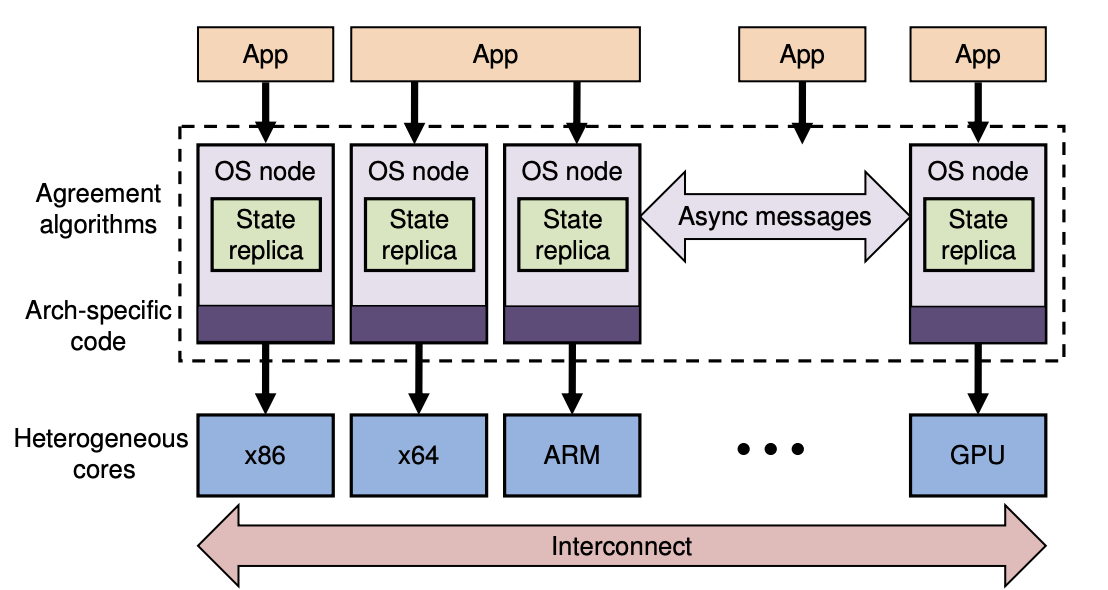
\includegraphics[width=0.6\textwidth]{Multi-kernel}
  \caption[Multi-kernel]{The Multi-kernel model \cite{multi_kernel_first_paper}}
  \label{fig:AzeleaKNL}
  \end{figure}

\subsubsection{Benefits of Multi-kernels}
The following below highlights the major characteristics
of Multi-kernels. 

\begin{itemize}
  \item Ability to handle diverse set of cores: 
  \item Interconnect matters: 
  \item Messages cost less than shared memory:
\end{itemize}

\subsection{Implementation}
The following section mentions about the Multi-kernel
implementations. 

\subsubsection{Barrelfish}
Barrelfish\cite{multi_kernel_first_paper} is a multi-kernel operating system that consists of a small kernel 
running on each core. The kernels share no memory (even on 
machines with cache-coherent shared RAM). A CPU 
driver in Barrelfish represents a kernel when is ran 
on a given core. In a heterogeneous system the CPU 
driver would different based on the architecture
of the core. 
% Add image 

\subsection{Popcorn Linux} % 1 
% https://www.kernel.org/doc/ols/2014/ols2014-barbalace.pdf
Popcorn\cite{PopcornLinux} linux is a replicated-kernel OS based on Linux. Popcorn 
boots up multiple instances of Linux kernels on a 
multi-core hardware. Popcorn linux was evaluated 
based on the NAS benchmark \cite{NAS}. Popcorn 
linux uses a customized compiler based 
off LLVM which translates C/C++ applications 
into machine code for runtime execution and migration 
across multiple ISAs. Papers and sub projects 
derived from popcorn Linux: 
\begin{itemize}
  \item Aparapi: Applying Source Level Auto-Vectorization
  \item AIRA: A Framework for Flexible Compute Kernel Execution in Heterogeneous Platforms
  \item HEXO: Offloading HPC Compute-Intensive Workloads on Low-Cost, Low-Power Embedded Systems.
  \item H-Container: Enabling Heterogeneous-ISA Container Migration in Edge Computing.
  \item HeterSec: Software diversification using ISA heterogeneity
\end{itemize}


% Skim through all the papers published 
% In depth writing (Understand the analysis of the survey paper)
% todo add more context about approach 
% todo Add image 

\subsection{FusedOS}
% Todo what is ran on the light weight cores 
FusedOS was one of the first to combine 
linux with a LWK(Light weight kernel). FusedOS 
was assuming heterogeneous hardware architecture 
that consists of both a light weight and full 
weight cores. The full cores runs linux and 
is also responsible to partition hardware 
resources between itself and LWKs.
To execute an application the LWK requests 
hardware resources (i.e light weight cores and memory) 
from the FWK(Full weight Kernel, This refers to the 
linux kernel). The system calls are generated 
by the application and are forwarded to Linux 
which is then handled with LWK process. 
% todo look at Github implementation 

\subsection{IHK/McKernel}
IHK/McKernel is a multi-kernel approach 
which runs Linux and LWKs side by side on 
compute nodes. A low-level software infrastructure
which is present at the heart of the stack 
which is called Interface for Heterogeneous
Kernels (IHK). By using IHK it is 
possible to dynamically partition resources 
in a many-core environment. An IKC (Inter-Kernel 
communication) layer is also introduced upon which 
the system call delegation is implemented. 
McKernel is a light weight kernel written 
from scratch and designed for HPC. McKernel
retains a binary compatible ABI with Linux. 
It supports multi-threading with a simple 
round robin cooperative scheduler. 

% \subsection{mOS}
% mOS creates a m

\subsection{FFMK}
FFMK (Fast and fault tolerant Microkernel based system) which 
is designed for Exascale computing. It investigates 
the feasibility of a Microkernel based hybrid OS designed 
for HPC.It relies on a L4 microkernel and a para-virtualized
Linux instance (i.e L4Linux\cite{l4linux}).
The idea of FFMK is to run HPC application directly on 
L4 with transparent access to linux features by using 
L4Linux. The L4Linux user process can be decoupled 
from the linux kernel and moved to another core 
if required (i.e by using the L4 Thread).

% Analysis 
% - Build table as per the survey (Simplify)
% - Mention 2 Multi-kernels that support Uni-kernels

% \subsection{Hobbes}
% todo read: https://link.springer.com/chapter/10.1007/978-981-13-6624-6_15


% \subsection{Pisces/Kitten}

% \subsection{Kitten/Palacios}




% Major features 
% Implementation 
% upto 4 major ones 



% ------------------------------ Best suited for various architectures -----------------------------

\section[TAG based architecture survey]{TAG based architecture survey}   
The following was a survey conducted on existing TAG based implementations and the 
recent survey based on TAG based architectures \cite{acmTAGSurvey} published
in 2022 was a good staring point to understand about various implementations of TAG
based architectures with the high level merits and limitations. The following section 
provides our own version of the Survey to help decide the best implementations 
to answer the research questions (//TODO reference research questions chapter).

\subsection{Introduction to TAG based architectures}

Before deep diving into TAG based architecture implementations it is important to 
answer what is a TAG based architecture ? and the high level of various 
categories of various TAG based architectures.

Tagged architectures are a prominent class of hardware security primitives that augment data and code words
with tags. The tags, which function as the security metadata
about memory, are created before the program is loaded. 
Then, at runtime, the hardware enforces security policies on the tags to provide safety guarantees. 
The advantage being tags automate the secure and efficient management of security metadata. 

Tags policies as designed to address mostly:
\begin{itemize}
  \item Type and memory corruption
  \item Integer overflows
  \item Thread safety
  \item Buffer overflows
\end{itemize}

TAG policies can be categorized into 5 main categories which is:
\begin{itemize}
  \item Information-low control (IFC) policies
  \item Dynamic information-low tracking (DIFT) policies
  \item Capability models
  \item Programmable architectures
\end{itemize}

\subsection{Implementations}
 
According to the TAG based architecture survey \cite{acmTAGSurvey} there are 37 published
efforts on TAG based architectures over the past decade and 20 published efforts preceding that. 
The following below are relevant papers in relation to the research questions: 

\subsubsection{Timder V}
 Timber V\cite{weiser_timber-v_2019} is a tagged memory architecture for flexible and efficient isolation of code and data on 
 small embedded systems. The TAG isolation is augmented with a memory protection unit to isolate 
 individual processes. Timber V is compatible with existing code. The contributions of the paper 
 are: 
 \begin{itemize}
  \item Efficient tagged memory architecture for isolated execution on low-end processors. 
  \item Concept introduced called stack interleaving that allows efficient and dynamic memory management. 
  \item Lightweight shared memory between enclaves. 
  \item Efficient shared MPU (i.e Memory Protection Unit) design. 
 \end{itemize}

 \begin{figure}[htbp!] 
  \centering
  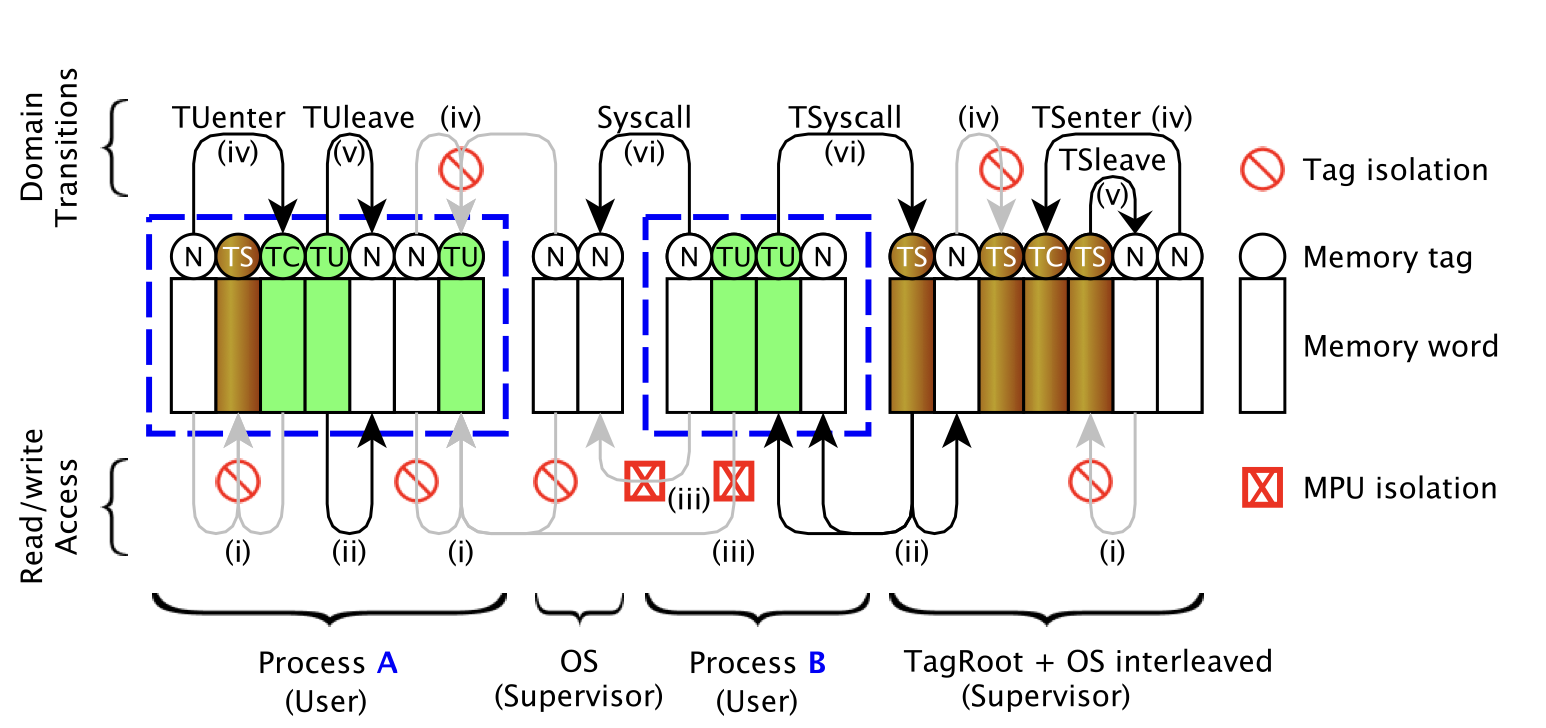
\includegraphics[width=0.6\textwidth]{Timber-V}
  \caption[MTE]{TimberV TAG interleaved on flat physical memory\cite{weiser_timber-v_2019}}
  \label{fig:MTE}
  \end{figure}
	
\subsubsection{ARM MTE}
The ARMv8.5-Memory Tagging Extension (MTE)\cite{ARMMTE} aims to increase the memory safety written for 
unsafe languages without requiring source code changes and in certain cases without 
recompilation. It generally focuses on the bounds checking use case, Though it 
provides limited tags which means it can only provide probabilistic overflow detection. 
It is one of the latest commercial incarnations of memory-safety-focused tagged architectures.   

\begin{figure}[htbp!] 
  \centering    
  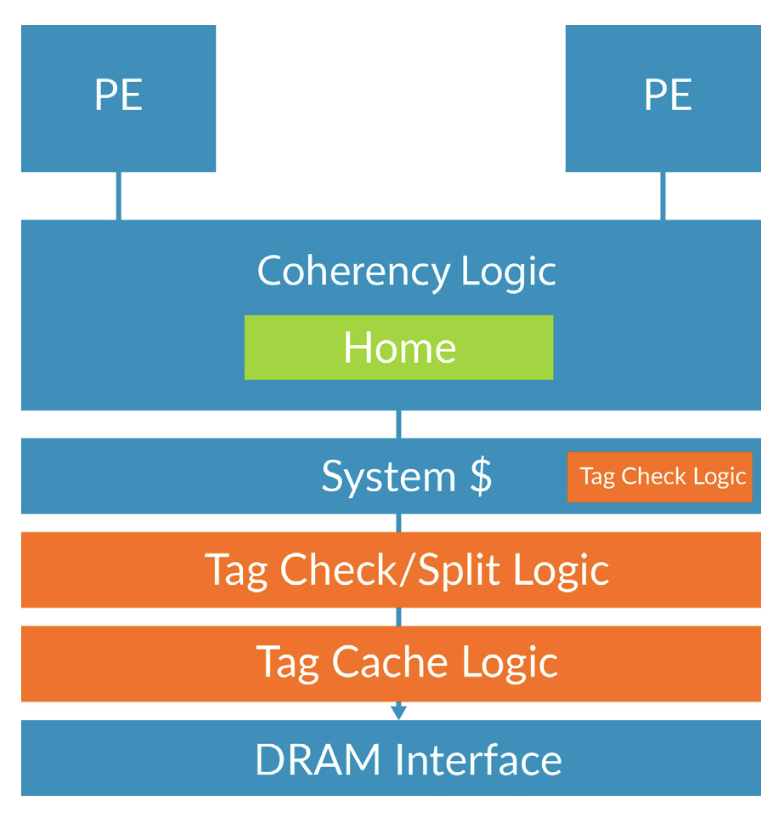
\includegraphics[width=0.2\textwidth]{ARMMTE}
  \caption[MTE]{Example of an ARM MTE-based system \cite{ARMMTE}}
  \label{fig:MTE}
  \end{figure}

\subsubsection{D-RI5CY}
D-RISCY\cite{D-RISCY} provides a design a design and implementation of a hardware dynamic information flow 
tracking (DIFT) architecture for RISC-V processor cores. The paper presents a low 
overhead implementation of DIFT that is specialized for low-end embedded systems
for IOT applications. The following are high level contributions:
\begin{itemize}
  \item Design f D-RI5CY, A DIFT-protected implementation of the RI5CY processor core. 
        The paper implements the modification of the DIFT TAG propagation and TAG checking
        mechanism in a way that is transparent to the execution of the regular instructions. 
  \item Concept introduced called stack interleaving that allows efficient and dynamic memory management.
  \item Lightweight shared memory between enclaves.
  \item Efficient shared MPU (i.e Memory Protection Unit) design.
\end{itemize}

\begin{figure}[htbp!] 
  \centering    
  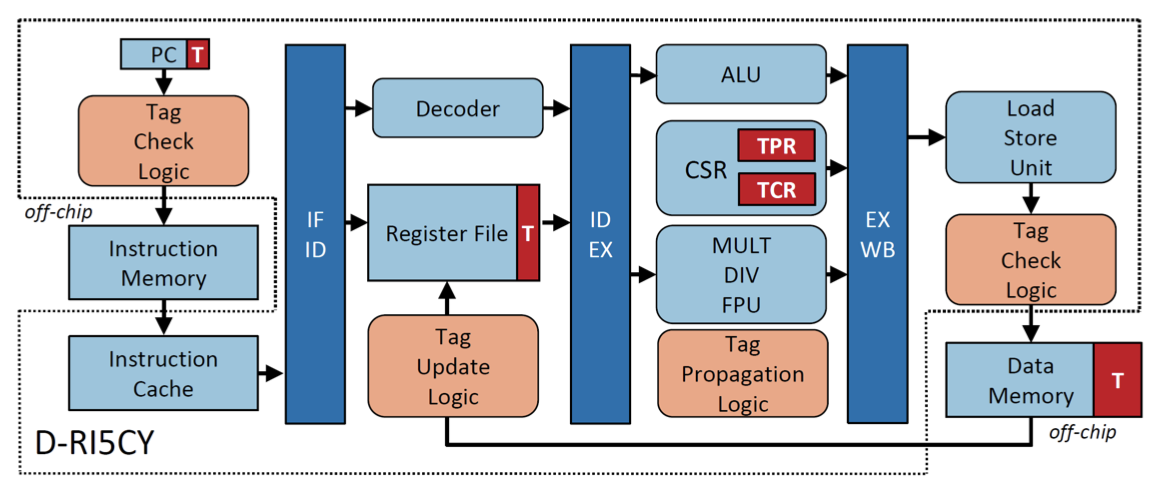
\includegraphics[width=0.6\textwidth]{D-RISCV}
  \caption[D-RISCY]{ Block diagram of the D-RI5CY processor. In red and pink the DIFT components. \cite{D-RISCY}}
  \label{fig:MTE}
  \end{figure}

%\subsection{TMDFI}


\subsubsection{HyperFlow} 
Hyperflow\cite{HyperFlow} is a design and security implementation that offers security assurance because it is implemented 
using a security-typed hardware description language. It allows complex information flow policies to 
be configured at run time. The paper introduces ChiselFlow, a new secure hardware description language. 
The contribution of the paper includes: 
\begin{itemize}
  \item Processor architecture and implementation designed for timing-safe information flow security. 
  \item Complete RISC-V instruction set extended with instructions for information flow control. 
  \item Verified at design time with a hardware description language. 
  \item Novel representations of lattices that can be implemented in hardware efficiently. 
\end{itemize}
HyperFlow implements a nonmalleable IFC policy using tags.
To eliminate timing side channels, the processor tracks the tag of the currently executing code and lushes caches,
TLB, branch predictor, and other micro-architectural state on changes in the conditionality or integrity tag of the
running code. The modifications to avoid timing side channels seem more extensive than those to add tags. The
authors report overheads in cycles per instruction of between 1\% and 69\%, largely due to padding the multiply
operation to the worst-case number of cycles.

\subsubsection{SDMP}
SDMP\cite{Sdmp} paper focuses on designing metadata tag based stack-protection security policies for general purpose tagged
architecture. The policies specifically
exploit the natural locality of dynamic program call graphs to
achieve cache-ability of the metadata rules that they require.
The simple Return Address Protection policy has a performance
overhead of 1.2\% but just protects return addresses.
The two richer policies present, Static Authorities and Depth Isolation, 
provide object-level protection for all stack objects. When
enforcing memory safety, The Static Authorities policy has a
performance overhead of 5.7\% and the Depth Isolation policy
has a performance overhead of 4.5\%.
The contribution of the paper includes:
\begin{itemize}
  \item The formulation of a range of stack protection policies
within the SDMP model.
  \item Three optimizations for the stack policies: Lazy Tagging,
Lazy Clearing and Cache Line Tagging.
  \item The performance modeling results of the policies on
a standard benchmark set, including the impact of the
proposed optimizations.
\end{itemize}

\subsubsection{Typed Architecture}
This paper introduces Typed
Architectures\cite{TypedArchitecture}, a high-efficiency, low-cost execution substrate 
for dynamic scripting languages, where each data
variable retains high-level type information at an ISA level.
Typed Architectures calculate and check the dynamic type
of each variable implicitly in hardware, rather than explicitly
in software. Typed Architectures provide
hardware support for flexible yet efficient type tag extraction
and insertion, capturing common data layout patterns of tag-
value pairs. The evaluation using a fully synthesizable RISC-
V RTL design on FPGA shows that Typed Architectures
achieve mean speedups of 11.2\% and 9.9\% with
minimum speedups of 32.6\% and 43.5\% for two production-
grade scripting engines for JavaScript and Lua. 
The contribution of the paper includes:
\begin{itemize}
  \item ISA extension to efficiently manage
type tags in hardware, which can be flexibly applied to
multiple scripting languages and engines.
  \item Design and implement the Typed Architecture pipeline,
which effectively reduces the overhead of dynamic type
checking at low hardware cost.
  \item Prototype the proposed processor architecture using 
a fully synthesizable RTL model to execute two
production-grade scripting engines with large inputs on
FPGA (executing over 274 billion instructions in total)
and provide a more accurate estimate of area and power
using a TSMC 40nm standard cell library.
\end{itemize}

\begin{figure}[htbp!] 
  \centering    
  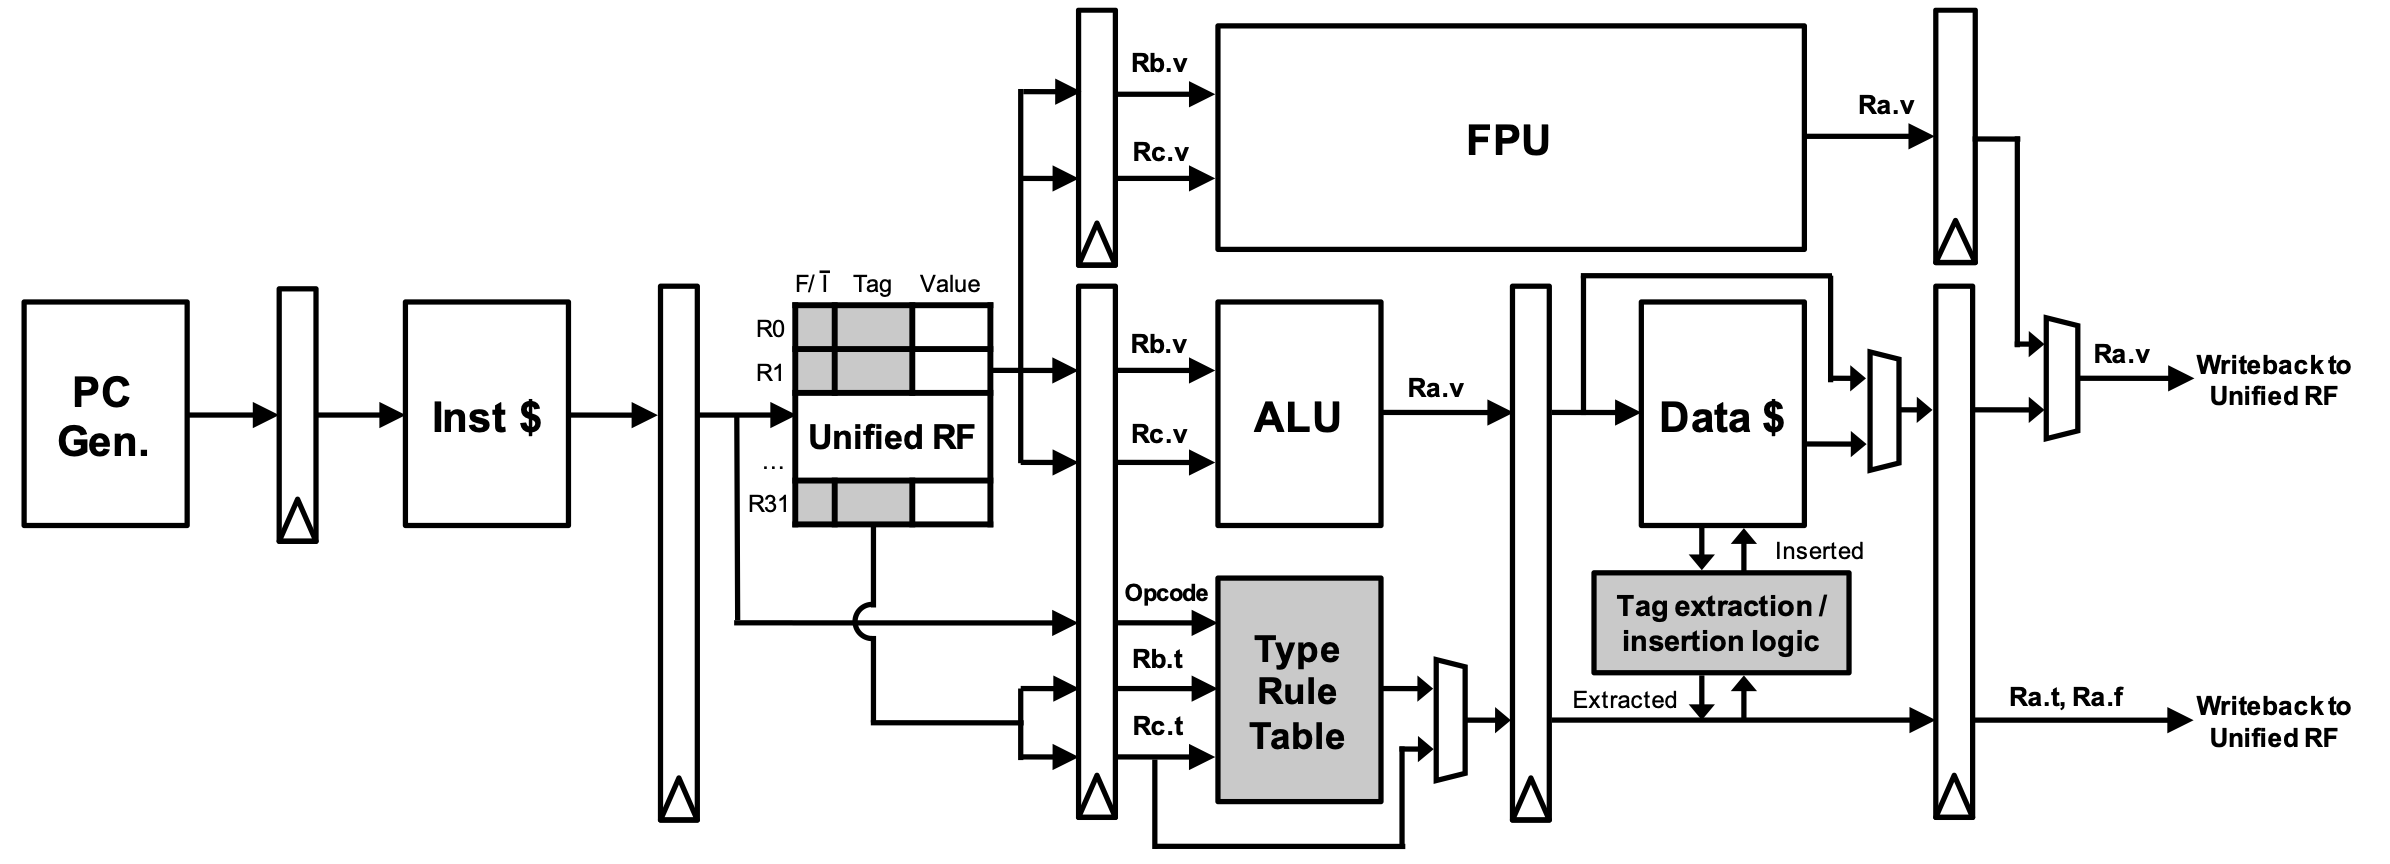
\includegraphics[width=0.8\textwidth]{TypedArchitecture}
  \caption[TypedArchitecture]{Pipeline structure augmented with Typed Architecture \cite{TypedArchitecture}}
  \label{fig:TypedArchitecture}
  \end{figure}

\subsubsection{Dover}
Dover\cite{Dover} is a secure processor that extends the conventional CPU with
a Policy Execution co-processor (PEX). PEX maintains metadata 
of every word assessable by the application processor. PEX 
enforces software-defined policies
at the granularity of each instruction executed by the AP(i.e application process)
CPU. Hardware interlocks enforce strict separation between code and data 
for user-land and policy-related. The Dover system has 
a dover specialized kernel and modifications to the GCC toolchain 
which can implement a wide range security and safety policies on 
top existing C based applications. 

\begin{figure}[htbp!] 
  \centering    
  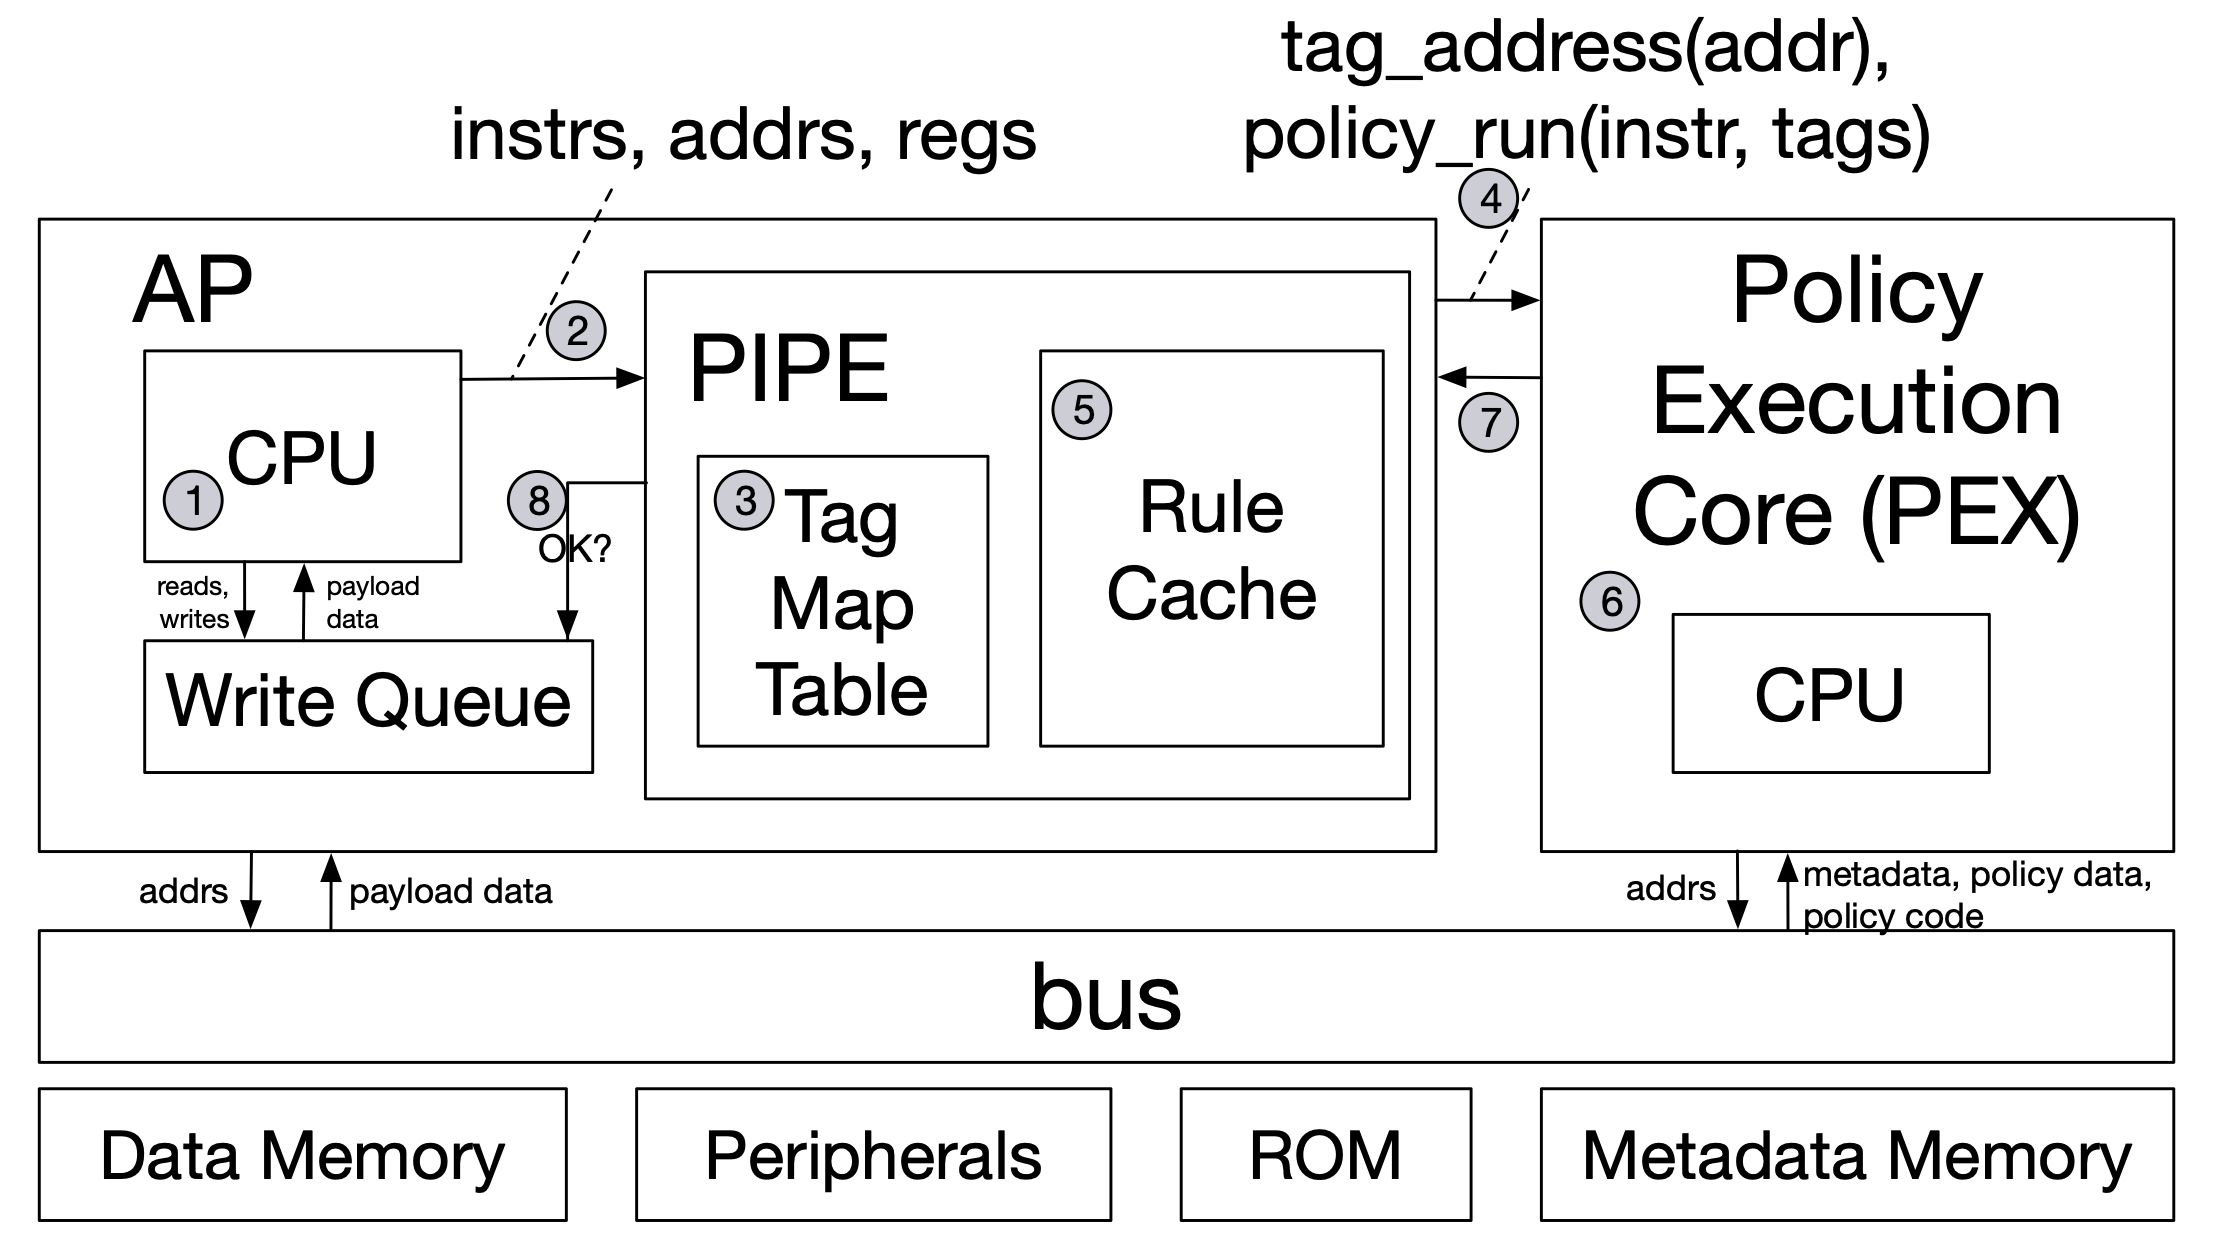
\includegraphics[width=0.8\textwidth]{Dover}
  \caption[Dover]{High level overview of Dover Architecture \cite{Dover}}
  \label{fig:Dover}
  \end{figure}x

%\subsection{Shakti-T}

%\subsection{HDFI}

%\subsection{lowRISC}

%\subsection{Taxi}

%\subsection{Pump}

\subsubsection{CHERI \cite{CHERI}}
CHERI (Capability Hardware Enhanced RISC Instructions) extends conventional processor
Instruction-Set Architectures (ISAs) with architectural capabilities to enable fine-grained
memory protection and highly scalable software compartmentalization. CHERI is a hybrid 
capability architecture that can combine capabilities with conventional MMU(i.e Memory Management
 Unit) based systems. The contribution of the following project include: 
\begin{itemize}
  \item ISA changes to introduce architecture capabilities.
  \item New microarchitecture proving that capabilities can be implemented efficiently 
        in hardware. Support for efficient tagged memory to protect capabilities and
        compress capabilities to reduce memory overhead.   
  \item Newly designed software construction model for that uses capability to provide
        fine grain memory protection and scalable software compartmentalization.  
  \item Language and Compiler extension to use capabilities for C and C++.
  \item OS extensions to use (and support application use of) fine-grained memory protection
        (spatial, referential, and (non-stack) temporal memory safety) and abstraction extensions
        to support scalable software compartmentalization. 
\end{itemize}

\begin{figure}[htbp!] 
  \centering    
  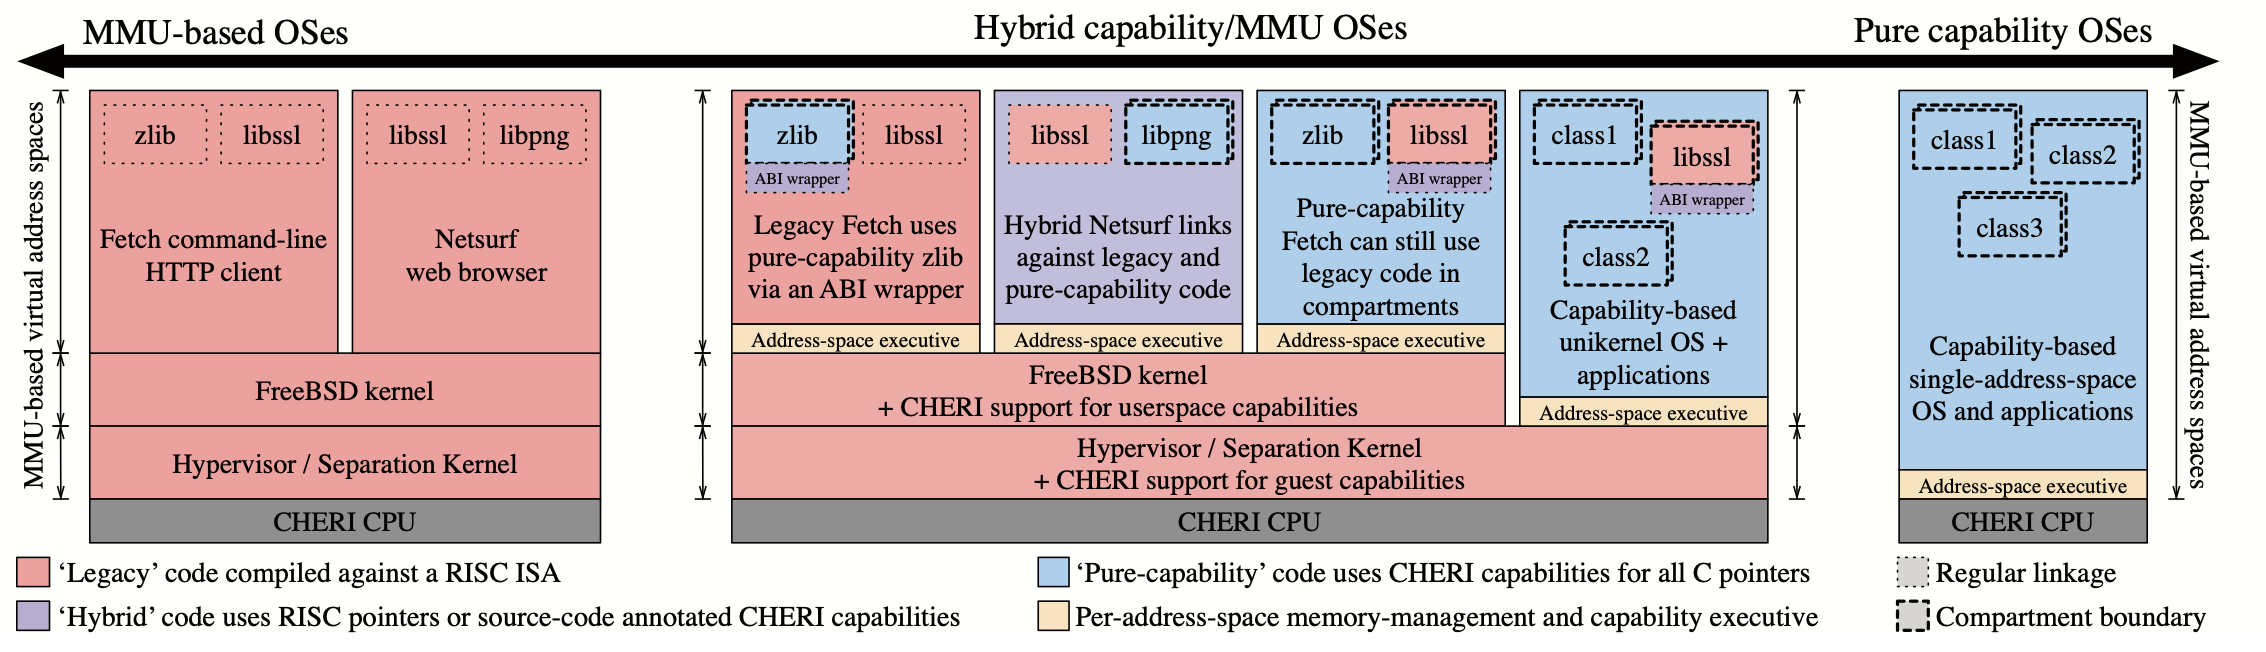
\includegraphics[width=0.9\textwidth]{Cheri}
  \caption[Cheri]{Spectrum of Hardware-software architectures, from conventional MMU-based virtualization and OS process models to single address-space capability system \cite{CHERI}}
  \label{fig:Cheri}
  \end{figure}
	
% \subsection{SPARC M7/M8 SSM}

\subsubsection{Low-Fat Pointers}
% https://dl.acm.org/doi/10.1145/2508859.2516713
Low-Fat Pointers\cite{LowFatPointer} adds hardware-managed tags to the pointer. 
This, in turn, allows the pointers to be used as capabilities to facilitate fine-grained 
access control and fast security domain crossing. The dedicated checking hardware runs in parallel 
with the processor's normal data-path so that the checks do not slow down processor operation 
(0\% runtime overhead).The following paper has a gate-level implementations of the logic for updating 
and validating these compact fat pointers and show that the hardware requirements are low 
and the critical paths for common operations are smaller than processor(i.e ALU operations).
The contribution of the following project include: 
\begin{itemize}
  \item Design and evaluation of a new, compact fat-pointer
  encoding and implementation (BIMA).
  \item Hardware that enforces the BIMA bounds checking and update, making the fat pointers 
  unforgeable and non-bypass able.
  \item Pipeline organization that allows the BIMA encoding to run just as fast as the baseline
   processor without spatial safety checking.
\end{itemize}


%\subsection{SAFE}

%\subsection{DataSafe}

%\subsection{Harmoni}

%\subsection{Shioya, et al.}

%\subsection{SIFT}

%\subsection{FlexCore}

%\subsection{Execution Leases}

%\subsection{GLIFT}

%\subsection{TIARA}

%\subsection{DIFT Coprocessor}

\subsubsection{HardBound}
% https://acg.cis.upenn.edu/papers/asplos08_hardbound.pdf
HardBound\cite{Hardbound} focuses on an architectural hardware bounded pointer primitive 
that supports hardware and software enforcements for memory safety in C programs. 
The C pointer representation is left intact but the bounds information is maintained 
separately and invisibly by the hardware. This means the bounds are initialized by 
software and is then propagated and transparently maintained by hardware (which automatically 
checks a pointer bound before it's dereferenced). The paper combined intra-procedural compiler 
instrumentation and hardware bounded pointers to enable a low overhead approach to enforce 
complete spatial memory safety in unmodified C programs. Based on the experiments conducted 
on the following paper the runtime overhead was between 5\% to 9\%. The following does not provide 
full type safety, handling dangling pointers and uninitialized memory reads.
The contribution of the following project include: 
\begin{itemize}
  \item A hardware bounded pointer primitive and accompanying complier transformation 
  that when combined enforce spatial safety for C programs. This is to minimize changes 
  to the compiler infrastructure and to retain compatibility with legacy C code. 
  \item Efficient implementation of hardware bounded pointers: This means using a compressed 
  metadata encoding, the entire base and metadata for bounds are stored in a reserver portion 
  of virtual memory. The hardware encodes the bounded pointer metadata by using just a few bits.
  These bits can be stored either in memory or unused bits in the pointer itself.
  \item Experimentally evaluating functional correctness and performance of the approach 
  in this paper.
\end{itemize}

% Analysis 
% - Similar to the Survey (Important architecture supported)
% - Comparing a security based TAG based architecture to performance 
% based one.  

% Mentioning all the comparisons 
% https://www.ssrg.ece.vt.edu/papers/hpdc19.pdf


% Main analysis iterate over the research questions 
% - Security Gurantees of Uni-kernels 
% - Security provided by TAG 
% - 

% Evaluation (Hierarchy evaluation based on diagram provided in Survey)
% Choose either performance or Security 


% Concrete evaluation bring all together 
% - Combining multi-kernel with efficiency of Uni-kernels with Custom hardware to for type system checking.\\
% - Analyzing memory interleaving is also of interest. 

% Prove choice of CHERI

\subsection{TAG based architecture analysis}

% Please add the following required packages to your document preamble:
% \usepackage{booktabs}
\begin{landscape}
\begin{table}[]
  \centering
  \caption{Analyzing various TAG-based implementations}
  \begin{tabular}{@{}lllllll@{}}
  \toprule
  \textbf{Architecture} & \textbf{Policy Goal} & \textbf{Complier} & \textbf{Bootloader} & \textbf{OS kernel} & \textbf{Processor} & \textbf{Evaluation} \\ \midrule
  Timder V              & IFC                  & Yes               & Yes                 & Yes                & Yes                & Simulation          \\
  ARM MTE               & Memory Safety        & Yes               & Yes                 & Yes                & Yes                & ASIC                \\
  D-RI5CY               & DIFT                 & Yes               & Yes                 & Yes                & Yes                & FPGA                \\
  HyperFlow             & IFC                  & No                & No                  & No                 & Yes                & FPGA                \\
  SDMP                  & Memory Safety        & Yes               & Yes                 & No                 & Yes                & Simulation          \\
  Typed Architecture    & N/A (Performance)    & Yes               & Yes                 & Yes                & Yes                & FPGA                \\
  Dover                 & Programmable         & Yes               & Yes                 & No                 & Yes                & FPGA                \\
  CHERI                 & Programmable         & Yes               & Yes                 & Yes                & Yes                & ASIC                \\
  HardBound             & Memory Safety        & Yes               & Yes                 & Yes                & Yes                & Simulation          \\ \bottomrule
  \end{tabular}
  \end{table}
\end{landscape}




%\subsection{Loki}

%\subsection{FLexiTaint}

%\subsection{SECTAG}

%\subsection{Raksha}

%\subsection{SecureBit}

%\subsection{Minos}

% \subsection{DIFT}
% The following paper provides simple architectural mechanism called dynamic information 
% flow tracking. DIFT protects programs from malicious attacks by identifying phony information 
% from untrusted I/O and restricting the usage of the phony information.

%\subsection{RIFLE}

%\subsection{AEGIS}

%\subsection{Mondriaan}

%\subsection{Aries}

%\subsection{XOM}

%\subsection{M-Machine}

%\subsection{KCM}

%\subsection{SPUR}

%\subsection{Lisp Machine}

%\subsection{HEP}

%\subsection{Burroughs}







































% %!TEX root = ../thesis.tex
%*******************************************************************************
%*********************************** Expirements *****************************
%*******************************************************************************

\chapter{Year 1 Activity}  %Title of the Year 1 Activity
This is section will be split into the timeline of activities of year 1.

\subsection{Poster SISCA PhD Conference}
The PhD symposium was held in in Glasgow Caledonian University for 2 days. A poster 
by the title "Benchmarking Unikernels with distributed map reduce"\cite{Sisca2022Poster}. The
objective for attending this conference was to socialize with other PhD students 
in Scotland by also presenting one of the plans of the initial experiments. 

Submission type:
\begin{enumerate}
    \item Poster: "Benchmarking Unikernels with distributed map reduce"\cite{Sisca2022Poster}
\end{enumerate}

\subsection{Europar PhD symposium and poster session}
The Europar PhD conference was held in the university of Glasgow. The title 
of the symposium paper being "Benchmarking Parallelism in Unikernels"\cite{Europar2022Paper}. This 
is expected to be published in springer proceeding of Europar 2022. 

Submission type:
\begin{enumerate}
    \item Poster: "Benchmarking Parallelism in Unikernels"\cite{Europar2022Poster}
    \item PhD Symposium paper: "Benchmarking Parallelism in Unikernels"\cite{Europar2022Paper}
\end{enumerate}
%!TEX root = ../thesis.tex
%*******************************************************************************
%*********************************** Research Timelines *****************************
%*******************************************************************************

\chapter{Research Timeline}  %Title of the Research Timeline
%!TEX root = ../thesis.tex
%*******************************************************************************
%*********************************** Conclusion *****************************
%*******************************************************************************

\chapter{Conclusion}  %Title of the Conclusion
This report provides a proposal for the potential research 
activities for the following. The main focus would be 
the literature review section which covers most of important 
bits of the following report. Based on the surveyed implementation 
in the literature review which is for Uni-kernels, Multi-kernels 
and TAG based architecture. The mappings about the following 
for Uni-kernels the best implementation of among the uni-kernel 
implementations surveyed would Hermit-Core, For Multi-kernels 
Popcorn linux would be suitable choice and for TAG based architecture
CHERI would be a suitable. Referring to the literature review 
provides the exact reasons. The research timeline section helped
more create focused depth of the initial milestones for the research 
activities to be conducted.
% \include{Chapter1/chapter1}
% \include{Chapter2/chapter2}
% \include{Chapter3/chapter3}
%\include{Chapter4/chapter4}
%\include{Chapter5/chapter5}
%\include{Chapter6/chapter6}
%\include{Chapter7/chapter7}



% ********************************** Back Matter *******************************
% Backmatter should be commented out, if you are using appendices after References
%\backmatter

% ********************************** Bibliography ******************************
\begin{spacing}{0.9}

% To use the conventional natbib style referencing
% Bibliography style previews: http://nodonn.tipido.net/bibstyle.php
% Reference styles: http://sites.stat.psu.edu/~surajit/present/bib.htm

\bibliographystyle{apalike}
%\bibliographystyle{unsrt} % Use for unsorted references  
%\bibliographystyle{plainnat} % use this to have URLs listed in References
\cleardoublepage
\bibliography{References/references} % Path to your References.bib file
% \bibliography{References/TAG-based-architecture/TAG-based-architecture} % Path to your References.bib file


% If you would like to use BibLaTeX for your references, pass `custombib' as
% an option in the document class. The location of 'reference.bib' should be
% specified in the preamble.tex file in the custombib section.
% Comment out the lines related to natbib above and uncomment the following line.

%\printbibliography[heading=bibintoc, title={References}]


\end{spacing}

% ********************************** Appendices ********************************

\begin{appendices} % Using appendices environment for more functunality

% \include{Appendix1/appendix1}
% \include{Appendix2/appendix2}

\end{appendices}

% *************************************** Index ********************************
\printthesisindex % If index is present

\end{document}
